\subsection*{Abstract}
Non-interference\index{non-interference} is an information flow policy\index{information flow!policy}
for guaranteeing confidentiality\index{confidentiality},
\ie that effects of sensitive data are not exposed to lower-level users, even
indirectly. When phrased in terms of programming languages, non-interference is
studied by attaching security classes\index{security class} to variables, then analyzing the classes
to determine if a violation, or a data \enquote{leak}, can occur. Security type
systems\index{security type system} are common controls for analyzing and enforcing non-interference.
Unfortunately, they require inference algorithms, program-level security
specifications, non-standard compilers, and are generally too restrictive or
complex for practical implementation. In this paper, we present a program logic
\lname that guarantees the semantic security property of \emph{anytime
non-interference}\index{non-interference!anytime}. By anytime, we mean a malicious actor with low-level access
cannot infer anything about higher-level values at any point of the program
execution. The logic links non-interference violations precisely to the faulty
commands and violations cannot be erased by program composition. We draw rich
inspiration from complexity-theoretic flow calculi, but obtaining a logic for
security analysis required significant adjustments. Finally, we share a
prototype to demonstrate \lname can be implemented as an automatic,
annotation-free, static security analyzer to obtain confidentiality guarantees
in practice.

\subsection{Introduction}
\label{subsec:ni-introduction}

Verifying that data is handled securely during computation is challenging
because it requires information beyond the program syntax. For example, consider
a hash function that computes a checksum of its input. Assume there exists a
malicious actor who can observe outputs of the hash function. If all inputs are
public data, we can guarantee the function does not expose secrets to the actor.
However, if we change the inputs to secret data, like social security numbers,
we no longer have the same guarantee for the same function. The hash function
then \enquote{leaks} information that possibly enables the actor to recover the
secret data.

\emph{Non-interference}~\cite{goguen1982}\index{non-interference} is a classical semantic security
property that constrains information flow\index{information flow} during computation. It is a mechanism
to enforce \emph{confidentiality}\index{confidentiality}, \ie concealment of information or resources
from unauthorized parties~\cite{bishop2003}. Non-interference\index{non-interference} is an attractive
target of study because it offers strong end-to-end guarantees for data
protection, it is inherently compositional, and can be enforced with program
logics or security type systems~\cite{cecchetti2017,frumin2021}\index{security type system}. Informally, a
program is non-interfering when secret data does not affect calculation of its
public outputs~\cite{sabelfeld2003}. In other words, data can only stay at the
same security class\index{security class} or flow to higher classes. Although a desirable property,
non-interference\index{non-interference} is in general undecidable by Rice's Theorem~\cite{rice1953}\index{Rice's Theorem} and
constructing a system that completely adheres to non-interference\index{non-interference} is overly
restrictive to capture real-world security
requirements~\cite{bossi2005,cecchetti2017}. However, unattainability of an
ideal construction does not restrict analysis of imperfect systems. Program
analysis enables detecting information flow\index{information flow} issues, supports informed
assessments of vulnerabilities, and identifies potential mitigations.

Our work extends the analysis of non-interference\index{non-interference} in theoretical directions
while yielding practical advantages. In literature, terminology around
non-interference\index{non-interference} is defined somewhat fluidly~\cite{sabelfeld2003}; admitting
multiple different but related {formal definitions}~\cite{nelson2020}, and
generalizing to the informal description provided previously. In this paper, we
introduce the notion of \emph{anytime non-interference}\index{non-interference!anytime}.
The anytime property is
powerful because it accounts for intermediate states of computation. Thus, it is
strictly stronger than the classic non-interference that is expressed in terms
of inputs and outputs. To lift our theory toward the real world, we provide our
main result: a program logic \lname that enables lightweight automatic static
program analysis of anytime non-interference\index{non-interference!anytime}.
We demonstrate practicality of
\lname through examples, a prototype implementation, and discussions of how
anytime non-interference\index{non-interference!anytime} elegantly supports numerous program analysis
applications.

Anytime non-interference\index{non-interference!anytime} tracks potential information flow\index{information flow} leaks in every legal
program state. A non-interfering program can be interrupted arbitrarily without
compromising its non-interference\index{non-interference} guarantee. Conversely, once a violating
operation has occurred, it is impossible to erase it. We consider time as
updates of public variable values. In other words, the latency between public
variable updates is instant. A change between two secret values, that causes a
loop to iterate longer according to a physical clock, has no observable side
effect. In general, anytime non-interference\index{non-interference!anytime} models security at the abstraction
level of programming languages and excludes lower-level execution details.
However, we consider the approach justified because potential information flow\index{information flow}
issues are often detectable from syntax.
 
Anytime non-interference\index{non-interference!anytime} is furthermore \emph{termination-insensitive}\index{non-interference!termination-insensitive}. Because
information signaled through termination can leak secrets indirectly,
termination\index{termination} handling is an ongoing design challenge for non-interference\index{non-interference}
systems~\cite{bay2020}. Untrusted programs, that pose high security risks,
require strong \emph{progress-sensitive} non-interference\index{non-interference!progress-sensitive} that considers both
termination and I/O interactions~\cite{hedin2012}. Trusted programs, with
predictable run-time behavior, permit weaker security checks and
termination-insensitivity\index{non-interference!termination-insensitive}.
Unfortunately, the binary situation provides no
middle ground for programs that mix trusted and untrusted code, \eg by dynamic
code loading\index{dynamic code loading}. In \autoref{subsub:termination} we discuss how to address this
limitation by partitioning computations based on security classes\index{security class}. This hybrid
approach relaxes the limitations of termination-insensitivity\index{non-interference!termination-insensitive} and monolithic
termination handing\index{termination}.

\subsubsection{The Essential Security Terminology Decoded}
\label{subsubsec:ni-terms}

Our work belongs to the domain of \emph{language-based
security}~\cite{schneider2001,sabelfeld2003}, where programming languages
principles (semantics, analysis, type systems, rewriting, \etc) are used to
strengthen application security. The \lname logic draws rich inspiration from
implicit computational complexity (refer to~\autoref{subsec:ni-related-works}), and
has applications in static program analysis; thus our work intersects many
related fields. Although we assume prior familiarity with logic and programming
languages, we define the relevant security concepts in this section.

\emph{Information flow}\index{information flow} denotes an observable action between two agents \(A\)
and \(B\). If an action performed by \(A\) is observable to \(B\), then there
exists an information flow from \(A\) to \(B\). The flow is \emph{explicit}\index{information flow!explicit} if
it is directly observable from a single action. The flow is \emph{implicit}\index{information flow!implicit} when
it is not directly observable, but reveals deductively the initial performed
action, after a sequence of other actions. To represent information flow, we
manipulate the conventional lattice\index{lattice} model à la Denning~\cite{denning76}.

An \emph{information flow policy}\index{information flow!policy} is a statement of what is, and what is not,
permissible~\cite{bishop2003} for a program \prc|C| in terms of flow between its
variables; formally defined as follows:

\begin{definition}[Information Flow Policy~\protect{\cite{volpanoI1996}}, Class
Assignment]\label{def:ifp} An \emph{information flow policy}\index{information flow!policy} is a lattice\index{lattice} \(\SC
= (\SCset, <)\) where \(\SCset\) is a partially \(<\)-ordered finite set of
\emph{security classes}\index{security class}.

We write \(\ell\) for the class assignment that assigns statically and
definitely to each variable \prc|x| occurring in a program \prc|C| its security
class \(\lvl{\prc|x|} \in \SC\). \end{definition}

By abuse of notation, we assume that a class assignment always comes with an
information flow policy\index{information flow!policy}, we write \(c \in \SC\), and for any two classes
\(c_1\), \(c_2\), we write \(c_1 \leqslant c_2\) if \(c_1 < c_2\) or \(c_1 =
c_2\), and \(c_1 \orth c_2\) if  \(c_1 \nleqslant c_2\) and \(c_2 \nleqslant
c_1\)--in this case, we say that \(c_1\) and \(c_2\) are \emph{orthogonal}.

A simple policy\index{information flow!policy} has two security classes\index{security class}, \eg \(\LH=(\{\scl{l}, \scl{h}\},
\{\scl{l} < \scl{h}\})\)---for \emph{low} and \emph{high}; but a policy can be
arbitrarily complex (refer to \autoref{ex-hasse-diagram-HMO}, located in
Appendix, for a more concrete example). We generally use a Hasse diagram\index{Hasse diagram} to
represent the information flow policy\index{information flow!policy} and class assignment in a compact manner,
as follows:

\begin{center}
\begin{minipage}{.68\textwidth}
\begin{alignat*}{7}
& \SCset = \{b, m_1, m_2, t\} \span \span \\ % \span are here to "ignore" the & alignment
& b < m_1 & \hspace{1.6em} & b < m_2 & \hspace{1.6em} & m_1 < t &\hspace{1.6em} & m_2 < t\\
& \lvl{\prc|x|} = b && \lvl{\prc|y$_1$|} = m_1 && \lvl{\prc|y$_2$|}= m_2 && \lvl{\prc|w|} =  \lvl{\prc|z|}  = t
\end{alignat*}
\end{minipage}\hfill%
\begin{minipage}{.3\textwidth}\hfill%
\begin{tikzpicture}[anchor=base, baseline=1.7em, node distance=1.6cm]
\node (b) {\(\lvl{\prc|x|}\)};
\node (m1) [above left of = b]  {\(\lvl{\prc|y$_1$|}\)};
\node (m2) [above right of = b] {\(\lvl{\prc|y$_2$|}\)};
\node (t) [above right of = m1] {\(\lvl{\prc|w|} = \lvl{\prc|z|}\)};
\draw[->] (b) -- (m1);
\draw[->] (b) -- (m2);
\draw[->] (m1) -- (t);
\draw[->] (m2) -- (t);
\end{tikzpicture}
\end{minipage}
\end{center}

An \emph{information flow control}\index{{information flow!control}} (IFC) is a mechanism to enforce a
policy~\cite{bishop2003}. Security type systems\index{security type system} (presented in
\autoref{sec:related-works}) are an example of a programming languages based
IFCs. They enforce a policy by annotating a program with security types\index{security type}. Then,
to be secure, a program must pass a compile-time type check. A sound IFC
guarantees to find all policy violations and a precise IFC avoids raising
excessive false alarms.

Formal security analysis uses the terms system model, security objective, and an
attacker model~\cite{bau2011,bognar2022}\index{attacker model}.
Our \emph{system model}\index{system model}, \ie the
system we want to secure, is a sequential imperative program, as specified
in~\autoref{subsec:language}, with effectful function calls discussed in
\autoref{sec:fct-calls}. Our \emph{security objective}\index{security objective},
\ie the system behaviors
that are considered secure, is defined by anytime non-interference\index{non-interference!anytime}
(\autoref{def:com-ni}). An \emph{adversary} is a malicious actor who poses a
threat to the system. An \emph{attacker model} specifies the capabilities and
motivations of the adversary. We assume a
\emph{program-centric}~\cite{hedin2012} attacker model\index{program centric attacker model}, where the adversary can
\begin{enumerate*}[label=(\roman*)]
\item see the program syntax
\item control public inputs and observe public outputs, and
\item up to the attacker's security class\index{security class}, access memory registers after updates.
\end{enumerate*}

\subsubsection{Contributions}
Our contributions are three-fold.

\begin{enumerate}
\item The main result is a lightweight syntactic IFC logic \lname
(\autoref{ni-logic}), with a built-in automatable inference algorithm, that
captures the semantic property of anytime non-interference\index{non-interference!anytime}.

\item We introduce the definition of anytime non-interference\index{non-interference!anytime}
(\autoref{def:com-ni}), and prove its correspondence with \lname, that follows
from the fundamental theorem (\autoref{thm:corr}).

\item We demonstrate the promising practical utility of \lname
(\autoref{sec:apps}), to include by describing our prototype static analyzer
\tool for analysis of \texttt{Java} programs. \end{enumerate}

\autoref{sec:fct-calls} furthermore discusses in detail how our approach can
accommodate different treatments of functions with and without side effects\index{side effect}, and
\autoref{subsec:ni-examples} gathers additional examples to help understanding.

\subsection{High-level Overview}
\label{sec:overview}

We consider deterministic imperative programs, with conventional operational
semantics, and variables of basic data types (integers, strings, \etc).
Let our expository program be the one in~\autoref{lst:expository}.

\begin{center}
\begin{minipage}{\textwidth}
\captionsetup{type=lstlisting}
\whileinputlisting{ni-expo.while}
\captionof{lstlisting}[Expository program]{Expository program.}
\label{lst:expository}
\end{minipage}
\end{center}

In the program, certain data flows are potentially problematic. The assignment
\prc|x = y| is an instances of an explicit flow\index{information flow!explicit}, since there is a direct flow
from variable \prc|y| to \prc|x|. The control expressions \prc|z==1| and
\prc|x==1| represent implicit flows\index{information flow!implicit}. They reveal information over execution
paths, and indirectly expose values of the control statement variables.
Admissibility of these data flows depends on the security classes\index{security class} of the
variables, since non-interference\index{non-interference} forbids data flowing from higher classes to
lower or between orthogonal classes. A sound IFC detects such issues and raises
an alarm.

The logic \lname produces a matrix of coefficients by applying inference rules
to programs. In a single derivation, it captures dependencies between all the
program variables, for all execution paths and security classes\index{security class}. The matrix is
interpreted by matching the \emph{in-variables}, \prc|v|\(_{\text{in}}\) (rows),
with the \emph{out-variables}, \prc|v|\(_{\text{out}}\) (columns).
The coefficients indicate:

\begin{description}

\item[\(\nv\)] -- \emph{no \emph{(non-interference)\index{non-interference}} violation}, no dependency
from \prc|v|$_\text{in}$ to \prc|v|$_\text{out}$,

\item[\(\vi\)] -- a \emph{violation}---or \enquote{leak}, hence the symbol---,
if \(\lvl{\prc|v$_{\text{out}}$|} < \lvl{\prc|v$_{\text{in}}$|}\) or
\(\lvl{\prc|v$_{\text{out}}$|} \orth \lvl{\prc|v$_{\text{in}}$|}\).

\end{description}

The matrix of the expository program,
\begin{center}
$\begin{pNiceMatrix}[first-row,first-col]
        & \prc|x|  & \prc|y|  & \prc|z|              \\
\prc|x| & \nv      & \vi      & \nv                  \\
\prc|y| & \textcolor{dgrey!60}{\vi} & \nv & \nv \\
\prc|z| & \vi      & \vi      & \nv
\end{pNiceMatrix}$
\end{center}
expectedly shows \emph{potential} violations in from \prc|y| to \prc|x|
(explicit\index{information flow!explicit}, in gray here) and \prc|x| to \prc|y|, \prc|z| to \prc|x|, and \prc|z|
to \prc|y| (implicit)\index{information flow!implicit}. The matrix gives a summary of potential violations for
the program that induced it. Evaluating the matrix determines if the program is
non-interfering; or if there exists a class assignment that makes the program
non-interfering. The evaluation function is parametric on the policy, enabling
evaluation against different policies.

\subsection{The Non-interference Logic}%
\label{ni-logic}

\subsubsection{A Simple Imperative While Language}%
\label{subsec:language}

We use a simple imperative \prc|while| language, with semantics similar to
\texttt{C}. The grammar is given in \autoref{fig:grammar}. The language supports
arrays and we let \prc|for| and \prc|do...while| loops be represented using
\prc|while| loops. How function calls can be added is discussed in
\autoref{sec:fct-calls}. The language subsumes (up to \prc|letvar| construct)
the \enquote{core block-structured language}~\cite{volpanoI1996}, and it maps
easily to the core fragment of \texttt{C}, \texttt{Java}, and other imperative
programming languages.

\begin{figure}
\begin{align*}
\emph{var} \ ::={ } \ &
  \prc|i| \ | \cdots \ | \ \prc|t| %
  \ | \cdots \ | \ \prc|x$_1$| \ | \ \cdots \ | \ \emph{var}[\emph{exp}]
  \tag{Variable}
  \\
\emph{exp} \ ::={ } \ &
  \emph{var} \ |\ \emph{val} \ |\ \emph{op}\texttt{(}\emph{exp},
  \hdots,\emph{exp}\texttt{)} \tag{Expression}
  \\
\emph{com} \ ::={ } \ &
  \emph{var \;} \prc|=| \mathit{\; exp}\ |\  \prc|skip| \ | \ \prc|if| \emph{
  exp } \prc|then| \emph{ com } \prc|else| \emph{ com } \ | \ \prc|while| \emph{
  exp } \prc|do| \emph{ com} \ | \ \emph{com;com} \tag{Command}
\end{align*}%
\caption{A simple imperative \prc|while| language}%
\label{fig:grammar}
\end{figure}

A variable \prc|x|, \prc|y|, \prc|z|, \(\hdots\) represents either an
undetermined \enquote{primitive} data type, \eg not a reference variable, or an
array, whose indices are given by an expression. We reserve $\prc|t|$ for
arrays. An expression is either a variable, a value (\eg integer literal) or the
application to expressions of some operator \emph{op}, which can be \eg
relational (\texttt{==},  \texttt{<}, \etc) or arithmetic  (\texttt{+},
\texttt{-}, \etc). We let \prc|e| (\resp \prc|C|) range over expressions (\resp
commands). We also use compound assignment operators and write \eg \prc|x++| for
\prc|x+=1|. We assume commands to be correct, \eg with operators correctly
applied to expressions, no out-of-bounds errors, \etc. A \emph{program} \prc|C|
is a sequence of commands, each command being either an \emph{assignment}, a
\emph{skip}, a \emph{branching}, a while \emph{loop} or the \emph{composition of
two commands}. A program $\prc|C|'$ is \emph{a sub-program of \prc|C|}, denoted
\(\prc|C|' \subseteq \prc|C|\), if $\prc|C|'$ occurs verbatim in \prc|C|. We
also define the following sets of variables.

\begin{definition}[\(\Occ\), \(\Out\) and \(\In\)]%
\label{def:in-out-occ}
We define the \emph{variables occurring in an expression} \prc|e| by:
\[\begin{aligned}[t]
\Occ(\prc|x|) =\prc|x| &
\Occ(\prc|op(e$_1$, $\hdots$,e$_n$)|) = \cup_{i = 1}^n \Occ(\prc|e$_i$|) &
\Occ(\prc|t[e]|) =\prc|t| \cup \Occ(\prc|e|) &
\Occ(\emph{val}) =\emptyset
\end{aligned}\]
\noindent
The set \(\Occ(\prc|C|)\) (\resp $\Out(\prc|C|)$, $\In(\prc|C|)$) of variables
\emph{occurring} in (\resp \emph{modified} by, \emph{used} by) a program \prc|C|
is defined in \autoref{table:def-out-in-occ}. We let $|\Occ(\prc|C|)|$ be the
cardinal of \(\Occ(\prc|C|)\).
\end{definition}

\begin{table}
\begin{NiceTabularX}{\hsize}{@{}l|CCC@{}}
\toprule
Command \prc|C| & $\Out(\prc|C|)$  & $\In(\prc|C|)$ & $\Occ(\prc|C|)=\Out(\prc|C|) \cup \In(\prc|C|)$ \\
\midrule
\prc|x = e| & \prc|x| & $\Occ(\prc|e|)$ & \prc|x| $\cup \Occ(\prc|e|)$
\\ \midrule
\prc|t[e$_1$] = e$_2$| & \prc|t| & $\Occ(\prc|e$_1$|) \cup \Occ(\prc|e$_2$|)$ & \prc|t| $\cup \Occ(\prc|e$_1$|) \cup \Occ(\prc|e$_2$|)$
\\ \midrule
\prc|skip| & $\emptyset$ & $\emptyset$ & $\emptyset$
\\ \midrule
\multicolumn{1}{@{}p{2.8cm}}{\prc|if e then C$_1$| \prc|else C$_2$|} & $\Out(\prc|C$_1$|) \cup \Out(\prc|C$_2$|)$ & $\Occ(\prc|e|) \cup \In(\prc|C$_1$|) \cup \In(\prc|C$_2$|)$ & $\Occ(\prc|e|) \cup \Occ(\prc|C$_1$|) \cup \Occ(\prc|C$_2$|)$
\\ \midrule
\prc|while e do C| & $\Out(\prc|C|)$ & $\Occ(\prc|e|) \cup \In(\prc|C|)$ & $\Occ(\prc|e|) \cup \Occ(\prc|C|)$
\\ \midrule
\prc|C$_1$;C$_2$| & $\Out(\prc|C$_1$|) \cup \Out(\prc|C$_2$|)$ & $\In(\prc|C$_1$|) \cup \In(\prc|C$_2$|)$ & $\Occ(\prc|C$_1$|) \cup \Occ(\prc|C$_2$|)$
\\
\bottomrule
\end{NiceTabularX}
\caption[Definition of $\Out$, $\In$ and $\Occ$ for commands]
{Definition of $\Out$, $\In$ and $\Occ$ for commands.}
\label{table:def-out-in-occ}
\end{table}

\subsubsection{Security-Flow Matrices for Non-interference Violation}
\label{subsec:sfg}\index{violation}

The \lname logic relies fundamentally on its ability to analyze data-flow
dependencies between variables occurring in commands. In this section, we define
the principles of this dependency analysis\index{dependence analysis}, founded on the theory of
\emph{security-flow matrices}, and how it maps to the presented language. This
dependency analysis is reminiscent of the one we developed to distribute
loops~\cite{aubert202213}. We assume familiarity with monoids and matrices
addition.

A security-flow matrix\index{security-flow matrix} $\sfm{\prc|C|}$ for a command \prc|C| is a hollow matrix
(\ie a matrix with only $\nv$ on the diagonal\footnote{This choice is clarified
after \autoref{def:violation}.}) over a monoid with an implicit choice of a
denumeration of \(\Occ(\prc|C|)\)\footnote{We will use the order in which the
variables occur in the program as their implicit order.}

\begin{definition}[Security monoid]\index{security monoid}
The \emph{security monoid} is \((\{\nv, \vi\}, \max)\), with \(\nv < \vi\).
\end{definition}

This monoid is isomorphic to the two-element Boolean algebra with only the
disjunction, with \(\vi\) representing a possible (non-interference) violation\index{violation}
that cannot be erased.

\begin{definition}[Security-flow matrix]\index{security-flow matrix}
\prc|C|, its \emph{security-flow matrix} $\sfm{\prc|C|}$ is a
$|\Occ(\prc|C|)|\times |\Occ(\prc|C|)|$ matrix over the security monoid\index{security monoid}, whose
construction is the object of \autoref{subsec:construction}.

For \(\prc|x|, \prc|y| \in \Occ(\prc|C|)\), we write
$\sfm{\prc|C|}(\prc|x|,\prc|y|)$ for the coefficient in $\sfm{\prc|C|}$ at the
row corresponding to the \emph{in-variable} $\prc|x|$ and column corresponding
to the \emph{out-variable} $\prc|y|$. \end{definition}

\begin{definition}[Violation]%
\label{def:violation}
Given \prc|C|, its security-flow matrix\index{security-flow matrix} $\sfm{\prc|C|}$ and a class assignment
\(\ell\), \prc|C| \emph{has a violation} if there exists \prc|x| and \prc|y|
such that $\sfm{\prc|C|}(\prc|x|,\prc|y|)=\vi$ and either \(\lvl{\prc|y|} <
\lvl{\prc|x|}\) or \(\lvl{\prc|y|} \orth \lvl{\prc|x|}\):

\begin{center}
$\begin{pNiceMatrix}[first-row,first-col]
        & \hdots  & \prc|y| & \hdots \\
\vdots  & \ddots  &         &  \iddots \\
\prc|x| &         & \vi     & \\
\vdots  & \iddots &         & \ddots
\end{pNiceMatrix}
\implies \prc|C| \text{ has a violation if }
\lvl{\prc|y|} < \lvl{\prc|x|}$ or $\lvl{\prc|y|} \orth \lvl{\prc|x|}$\text{.}\hfill
\end{center}
\end{definition}

Since \(\lvl{\prc|x|} < \lvl{\prc|x|}\) and $\lvl{\prc|x|} \orth \lvl{\prc|x|}$
are always false, there is no point keeping track of the values on the diagonal:
this is why hollow matrices are enough. This is also confirmed by the intuition:
it does not make sense to track data \enquote{leaking} from a variable to
itself.

How a security-flow matrix\index{security-flow matrix} is constructed by induction over the command is
explained in \autoref{subsec:construction}. To avoid resizing matrices whenever
additional variables are considered, we identify $\sfm{\prc|C|}$ with its
embedding in any larger matrix, \ie we abusively call the security-flow matrix
of \prc|C| any matrix containing $\sfm{\prc|C|}$ (up to rows swapping and
columns swapping) and containing \(\nv\) otherwise, implicitly viewing the
additional rows and columns as variables not occuring in \prc|C|. Visually, this
means that the following matrices are all viewed as $\sfm{\prc|C|}$ with
\(\Occ(\prc|C|)=\{\prc|x|, \prc|y|\}\) and $\sfm{\prc|C|}(\prc|x|,\prc|y|)=\vi$:
\begin{center}
\hfill
$\begin{pNiceMatrix}[first-row,first-col]
& \prc|x| & \prc|y|\\
\prc|x| &  \nv & \vi \\
\prc|y| & \nv & \cdot
\end{pNiceMatrix}$
\hfill
$\begin{pNiceMatrix}[first-row,first-col]
& \prc|y|  & \prc|x|  & \prc|z| \\
\prc|y| & \nv      &  \nv     & \nv \\
\prc|x| & \vi      &  \nv     & \nv \\
\prc|z| & \nv      &  \nv     & \nv
\end{pNiceMatrix}$
\hfill
$\begin{pNiceMatrix}[first-row,first-col]
& \prc|w| & \prc|x| & \prc|y|  \\
\prc|w| & \nv      &  \nv     & \nv \\
\prc|x| & \nv      &  \nv     & \vi \\
\prc|y| & \nv      &  \nv     & \nv
\end{pNiceMatrix}$
\hfill~
\end{center}
Continuing this example and using our compact presentation of information flow
policy\index{information flow!policy} and class assignment as single Hasse diagram\index{Hasse diagram}, \prc|C| would have a
violation with the level assignments
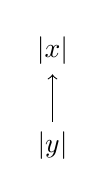
\begin{tikzpicture}[anchor=base, baseline=1.3em, node distance=1.2cm]
\node (y) {\(\lvl{\prc|y|}\)};
\node (x) [above of = y] {\(\lvl{\prc|x|}\)};
\draw[->] (y) -- (x);
\end{tikzpicture}
and
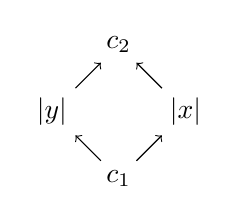
\begin{tikzpicture}[anchor=base, baseline=2.3em, node distance=1.2cm]
\node (c1) {\(c_1\)};
\node (y) [above left of = c1] {\(\lvl{\prc|y|}\)};
\node (x) [above right of = c1] {\(\lvl{\prc|x|}\)};
\node (c2) [above right of = y] {\(c_2\)};
\draw[->] (c1) -- (x);
\draw[->] (c1) -- (y);
\draw[->] (x) -- (c2);
\draw[->] (y) -- (c2);
\end{tikzpicture},
but would be free of violation with \(\lvl{\prc|x|} = \lvl{\prc|y|}\) or
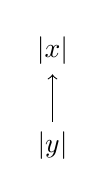
\begin{tikzpicture}[anchor=base, baseline=1.3em, node distance=1.2cm]
\node (y) {\(\lvl{\prc|y|}\)};
\node (x) [above of = y] {\(\lvl{\prc|x|}\)};
\draw[->] (y) -- (x);
\end{tikzpicture}.

\subsubsection{Constructing Security-Flow Matrices}%
\label{subsec:construction}\index{security-flow matrix}

The security-flow matrix of a command is constructed by induction, using the
security monoid\index{security monoid}. \autoref{subsec:ni-examples} gathers additional examples with
longer discussion.

\paragraph{Base Cases: Assignment and Skip} The security-flow matrix for an
assignment \prc|C| simply tracks flows from $\In(\prc|C|)$ to $\Out(\prc|C|)$:

\begin{definition}[Assignment]%
\label{def:assignment}
Given an assignment \prc|C|, we define \(\sfm{\prc|C|}\) by:
\[
\sfm{\prc|C|}(\prc|x|,\prc|y|)=
\begin{dcases*}
\vi & if $\prc|x| \in \In(\prc|C|)$, $\prc|y| \in \Out(\prc|C|)$ and $\prc|x| \neq \prc|y|$ \\
\nv & otherwise
\end{dcases*}
\]
\end{definition}

\begin{table}
\begin{tabularx}{\textwidth}{@{}llcX@{}}
\toprule
\prc|C| & $\Out(\prc|C|)$, $\In(\prc|C|)$
& $\sfm{\prc|C|}$ & \prc|C| has violation(s) if \ldots \\
\midrule
\prc|w = 3|
& %
$\begin{aligned}
\Out(\prc|C|) &=\{\prc|w|\}    \\
\In(\prc|C|)  &=\emptyset
\end{aligned}$
&
$\begin{pNiceMatrix}[first-row,first-col,baseline=t]
& \prc|w|\\
\prc|w| &  \nv
\end{pNiceMatrix}$
& (Impossible)
\\
\prc|y = x|
& %
$\begin{aligned}
\Out(\prc|C|) &=\{\prc|y|\}    \\
\In(\prc|C|)  &=\{\prc|x|\}
\end{aligned}$
& %
$\begin{pNiceMatrix}[first-row,first-col,baseline=t]
& \prc|y| & \prc|x|\\
\prc|y| &  \nv & \nv \\
\prc|x| & \vi & \nv
\end{pNiceMatrix}$
& \(\lvl{\prc|y|} < \lvl{\prc|x|}\) or \(\lvl{\prc|y|} \orth \lvl{\prc|x|}\).
\\
\prc|w = t[x + 1]|
& %
$\begin{aligned}
\Out(\prc|C|) &=\{\prc|w|\}    \\
\In(\prc|C|)  &=\{\prc|t|, \prc|x|\}
\end{aligned}$
& %
$\begin{pNiceMatrix}[first-row,first-col,baseline=t]
& \prc|w| & \prc|t| & \prc|x| \\
\prc|w| &  \nv & \nv & \nv\\
\prc|t| & \vi & \nv & \nv \\
\prc|x| & \vi & \nv & \nv
\end{pNiceMatrix}$
& $\begin{aligned}
\lvl{\prc|w|} &< \lvl{\prc|t|}\text{, }  & \lvl{\prc|w|} &\orth \lvl{\prc|t|} \text{,}\\
\lvl{\prc|w|} &< \lvl{\prc|x|}\text{ or\kern-1em} & \lvl{\prc|w|} &\orth \lvl{\prc|x|}\text{.}
\end{aligned}$\\
\prc|t[i] = u + j|
& %
$\begin{aligned}
\Out(\prc|C|) &=\{\prc|t|\}          \\
\In(\prc|C|)  &=\{\prc|i|, \prc|u|, \prc|j|\}
\end{aligned}$
& %
$\begin{pNiceMatrix}[first-row,first-col,baseline=t]
& \prc|t| & \prc|i| & \prc|u| & \prc|j| \\
\prc|t| &  \nv & \nv & \nv & \nv \\
\prc|i| & \vi & \nv & \nv & \nv \\
\prc|u| & \vi & \nv & \nv &\nv\\
\prc|j| & \vi & \nv & \nv & \nv
\end{pNiceMatrix}$
&  $\begin{aligned}
\lvl{\prc|t|} &< \lvl{\prc|i|}\text{,} & \lvl{\prc|t|} &\orth \lvl{\prc|i|}\text{,}\\
\lvl{\prc|t|} &< \lvl{\prc|u|}\text{,} & \lvl{\prc|t|} &\orth \lvl{\prc|u|}\text{,}\\
\lvl{\prc|t|} &< \lvl{\prc|j|}\text{ or\kern-.6em} & \lvl{\prc|t|} &\orth \lvl{\prc|j|}\text{.}
\end{aligned}$ \\
\bottomrule
\caption[Statement Examples, Sets, Representations of their Possible Violation(s)]
{Statement Examples, Sets, Representations of their Possible Violation(s).}
\label{tab:threecases}
\end{tabularx}
\end{table}

We illustrate in \autoref{tab:threecases} some basic cases: we consider an array
a single entity, and that changing one value in it means being able to access it
completely. More precisely, \prc|t[i]| on the left-hand side of an assignment is
a violation if \(\lvl{\prc|t|} > \lvl{\prc|i|}\) (\resp \(\lvl{\prc|t|} \orth
\lvl{\prc|i|}\)). Indeed, it implies that a lower-class (\resp orthogonal-class)
variable (\prc|i|) can decide where to write in a higher-class (\resp
orthogonal-class) variable (\prc|t|). However, \prc|t[i]| as an expression (\eg
on the right-hand side of an assignment or in a condition, as discussed in
\autoref{sssec:correction}) is acceptable as long as the variable(s) storing the
result of this calculation or dependent on that condition's truth value have
class higher or equal to \prc|t| and \prc|i| classes.

\begin{definition}[Skip]
We let $\sfm{\prc|skip|}$ be the matrix with $0$ rows and columns.
\end{definition}

Identifying $\sfm{\prc|skip|}$ with its embeddings, it is the empty matrix of
any size.

\paragraph{Composition as a Commutative Operation}

The security-flow matrix\index{security-flow matrix} for a composition of commands is an abstraction that
allows manipulating a sequence of commands as one command with its own matrix.

\begin{definition}[Composition]
We let $\sfm{\prc|C$_1$;$\cdots$;C$_n$|}$
be $\sfm{\prc|C$_1$|} + \cdots + \sfm{\prc|C$_n$|}$.
\end{definition}

\newsavebox\compone
\begin{lrbox}{\compone}
\begin{minipage}{.25\linewidth}
\begin{whilelisting}*[numbers=none]
w = w + x;
z = y + 2
\end{whilelisting}
\end{minipage}
\end{lrbox}

\newsavebox\comptwo
\begin{lrbox}{\comptwo}
\begin{minipage}{.25\linewidth}
\begin{whilelisting}*[numbers=none]
x = y * 2;
z = 0
\end{whilelisting}
\end{minipage}
\end{lrbox}

\begin{figure}
\begin{center}
\begin{tabular}{ccccc}
\prc|C$_1$| && \prc|C$_2$| && \prc|C$_1$;C$_2$| \\
$\begin{pNiceMatrix}[first-row,first-col,left-margin=-2pt,right-margin=-2pt]
        & \prc|w|  & \prc|x|  & \prc|y|  & \prc|z| \\
\prc|w| & \nv      & \nv      & \nv      & \nv     \\
\prc|x| & \vi      & \nv      & \nv      & \nv     \\
\prc|y| & \nv      & \nv      & \nv      & \vi     \\
\prc|z| & \nv      & \nv      & \nv      & \nv
\end{pNiceMatrix}$ & + &
$\begin{pNiceMatrix}[first-row,first-col,left-margin=-2pt,right-margin=-2pt]
        & \prc|w|  & \prc|x|  & \prc|y|  & \prc|z| \\
\prc|w| & \nv      & \nv      & \nv      & \nv     \\
\prc|x| & \vi      & \nv      & \nv      & \nv     \\
\prc|y| & \nv      & \vi      & \nv      & \vi     \\
\prc|z| & \nv      & \nv      & \nv      & \nv
\end{pNiceMatrix}$ & = &
$\begin{pNiceMatrix}[first-row,first-col,left-margin=-2pt,right-margin=-2pt]
        & \prc|w|  & \prc|x|  & \prc|y|  & \prc|z| \\
\prc|w| & \nv      & \nv      & \nv      & \nv     \\
\prc|x| & \vi      & \nv      & \nv      & \nv     \\
\prc|y| & \nv      & \vi      & \nv      & \vi     \\
\prc|z| & \nv      & \nv      & \nv      & \nv
\end{pNiceMatrix}$ \\ \\
\usebox\compone && \usebox\comptwo \\
\end{tabular}
\end{center}
\caption[Security-Flow Matrix of compositions]
{Security-Flow Matrix of compositions.}
\label{fig:composition}
\index{security-flow matrix}
\end{figure}

The composition of commands \prc|C$_1$| and \prc|C$_2$|---themselves already the
result of compositions of assignments involving disjoint variables---is
illustrated in~\autoref{fig:composition}. Two important observations:

\begin{enumerate}
\item
Some existing approaches might consider \prc|C$_1$;C$_2$| as free of violation
even if \(\lvl{\prc|z|} < \lvl{\prc|y|}\), since \(\prc|z = 0|\) will wipe out
the content of \prc|z| and \enquote{cancel} the violation introduced by \prc|z =
y|. The intuition is that an attacker observing the output (or even all the
final values) cannot deduce anything about \prc|z|'s value (and, transitively\index{information flow!transitive},
about the value of the higher-class \prc|y|) once the computation is over. Our
\enquote{once a violation, always a violation} approach ignores the fact that
\enquote{ultimately}, this violation may be hidden--the anytime non-interference\index{non-interference!anytime}
guarantee is discussed in \autoref{subsec:ni-soundness}.
\item
Interestingly, $\sfm{\prc|C$_1$;C$_2$|} = \sfm{\prc|C$_2$;C$_1$|}$ since
composition is interpreted as a sum of matrices over our \emph{commutative}
security monoid\index{security monoid}. While previous flow-based
approaches~\cite{aubert20222,aubert20232,jones2009} requires semi-ring because
composition was handled \emph{via} product of matrices, the current set-up
simplifies the machinery precisely to keep track of past violations.
\end{enumerate}

\paragraph{A Correction for Implicit Flows}%
\label{sssec:correction}

To account for implicit flows\index{information flow!implicit}, branchings and loops require a \emph{correction}.
The main idea is that interpreting \prc|if e then C$_1\;$ else C$_2$| (\resp
\prc|while e do C|) require to record that all the variables modified in
\prc|C$_1$| and \prc|C$_2$| (\resp in \prc|C|) depend on the variables
\emph{occurring} in \(\prc|e|\) (as opposed to the assignment considering the
variables \emph{used} by \prc|C|).

\begin{definition}[Correction]%
\label{def:correction}
The \emph{correction $\corr{\prc|e|}_{\prc|C|}$ of an expression \prc|e| on a
program \prc|C|} is
\[
\corr{\prc|e|}_{\prc|C|}(\prc|x|,\prc|y|)=
\begin{dcases*}
\vi & if $\prc|x| \in \Occ(\prc|e|)$, $\prc|y| \in \Out(\prc|C|)$ and \(\prc|x|
\neq \prc|y|\) \\
\nv & otherwise
\end{dcases*}
\]
\end{definition}

Intuitively, the correction states that if the variable \prc|y| is modified in
the body of either branch of the branching or in the body of the loop and
\(\prc|x|\) occurs in the expression, then there is a violation if
\(\lvl{\prc|y|} < \lvl{\prc|x|}\) or \(\lvl{\prc|y|} \orth \lvl{\prc|x|}\).

As an example, let us use \autoref{fig:composition} to construct \(\corr{\prc|w
> x|}_{\prc|C$_1$;C$_2$|}\), \eg \prc|w > x|'s correction for \prc|C$_1$;C$_2$|.
Variables \prc|w| and \prc|x|, through the expression \prc|w > x|, control the
values of \prc|w|, \prc|x| and \prc|z| since \prc|C$_1$| and \prc|C$_2$| set
those values, and their execution depend on it, giving:

\[\begin{pNiceMatrix}[first-row,first-col]
& \prc|w| & \prc|x| & \prc|y| & \prc|z|\\
\prc|w| & \nv & \vi & \nv & \vi \\
\prc|x| & \vi & \nv & \nv & \vi \\
\prc|y| & \nv & \nv & \nv & \nv \\
\prc|z| & \nv & \nv & \nv & \nv
\end{pNiceMatrix}.\]

Observe also that in \(\corr{\prc|t[i] != x|}_{\prc|C|}\) the variables \prc|t|,
\prc|i| and \prc|x| would be marked as controlling the variables occurring in
\(\Out(\prc|C|)\). However, no constraint would be imposed between the classes
of \prc|t|, \prc|i| and \prc|x|, since they would all be required to flow into
classes that are higher or equal to theirs.

\paragraph{Conditionals and Loops}
Following our previous observation, branchings and loops are interpreted
similarly.

\begin{definition}[Branching]%
\label{def:if}
We let $\sfm{\prc|if e then C$_1\;$ else C$_2$|}$
be $\sfm{\prc|C$_1$;C$_2$|} + \corr{\prc|e|}_{\prc|C$_1$;C$_2$|}$.
\end{definition}

\newsavebox\ifconectwo
\begin{lrbox}{\ifconectwo}
\begin{minipage}{4cm}
\lstinputlisting[mathescape,nolol,frame=none,numbers=none,aboveskip=0em,belowskip=0em]{if-else.while}
\end{minipage}
\end{lrbox}

\noindent
Adding \(\corr{\prc|w > x|}_{\prc|C$_1$;C$_2$|}\) to $\sfm{\prc|C$_1$|} +
\sfm{\prc|C$_2$|}$ from \autoref{fig:composition}, we obtain:
\[\mathbb{M} \left(~ \usebox\ifconectwo
\right) \ = \ \begin{pNiceMatrix}[first-row,first-col]
& \prc|w| & \prc|x| & \prc|y| & \prc|z|\\
\prc|w| & \nv & \vi & \nv & \vi  \\
\prc|x| & \vi & \nv & \nv & \vi \\
\prc|y| & \nv & \vi & \nv & \vi \\
\prc|z| & \nv & \nv & \nv & \nv
\end{pNiceMatrix}\text{.}\]

Observe that there is a violation if \(\lvl{\prc|w|} < \lvl{\prc|x|}\) or
\(\lvl{\prc|w|} \orth \lvl{\prc|x|}\) from the statement $\prc|w = w + x|$, and
that there is a violation if \(\lvl{\prc|x|} < \lvl{\prc|w|}\) or
\(\lvl{\prc|x|} \orth \lvl{\prc|w|}\). The latter comes from the fact that the
value of \(\prc|w|\) will decide if \(\prc|x = y * 2|\) will execute through the
expression. To be free of violations, such a program must be given a class
assignment satisfying \(\lvl{\prc|w|} = \lvl{\prc|x|}\) and the other
constraints recorded in the matrix.

\begin{definition}[Loop]
We let \(\sfm{\prc|while e do C|}\) be \(\sfm{\prc|C|} + \corr{\prc|e|}_{\prc|C|}\).
\end{definition}

\newsavebox\whilec
\begin{lrbox}{\whilec}
\begin{minipage}{4cm}
\lstinputlisting[mathescape,nolol,frame=none,numbers=none,aboveskip=0em,belowskip=0em]{arrays.while}
\end{minipage}
\end{lrbox}
\[\mathbb{M} \left(~ \usebox\whilec
\right) \ = \ \begin{pNiceMatrix}[first-row,first-col]
& \prc|t| & \prc|i| & \prc|j| & \prc|s1| & \prc|s2| \\
\prc|t| & \nv &\vi & \nv & \vi & \vi \\
\prc|i| & \nv & \nv & \nv & \vi & \vi \\
\prc|j| & \nv & \vi & \nv &\vi & \vi\\
\prc|s1| & \nv & \nv & \nv & \nv & \nv \\
\prc|s2| & \nv & \nv & \nv & \nv & \nv
\end{pNiceMatrix} \]

Since \prc|s1| and \prc|s2| do not control any other variable, their rows are
all $\nv$s. On the other hand, \prc|t|, \prc|i| and \prc|j| control the values
of \prc|s1|, \prc|s2| and \prc|i|, since they determine how many times the body
will execute.

\subsection{Capturing Anytime Non-Interference}%
\label{subsec:ni-soundness}\index{non-interference!anytime}

In the seminal work of Volpano et al.~\cite[pg.~173]{volpanoI1996},
\enquote{\textins{s}oundness \textins{wa}s formulated as a kind of
noninterference property. \textins{\dots I}f a variable $v$ has security
\textins{class $c$} , then one can change the initial values of any variables
whose security levels are not dominated by \textins{$c$} , execute the program,
and the \emph{final value} of $v$ will be the same, \emph{provided the program
terminates successfully}.} (our emphasis). \emph{Anytime non-interference}\index{non-interference!anytime},
defined below and captured by \lname, inspects the values \emph{while the
program is being executed}. It allows us to
\begin{enumerate*}
\item avoid making assumptions of program termination\index{termination}, or avoid waiting for
termination, and
\item model attackers who are capable of observing updates to variables at class
$c$ or lower.
\end{enumerate*}

First, we need to define a notion of \emph{timed} execution, which captures the
idea that an external observer can see updates on variables below a particular
security class\index{security class} in \enquote{real time}.

\begin{definition}[Timed command execution]
Given
\begin{enumerate}
\item a program \prc|C| with variables \(\prc|x|_1, \hdots, \prc|x|_n\),
\item a class assignment \(\ell : \Occ(\prc|C|) \to \SC\),
\item a security class\index{security class} \(\scl{c} \in \SC\),
\item a \emph{time (counter)} \(t \in \mathbb{N}\),
\item and a value list \(\vec{v} = v_1, \hdots, v_n\),
\end{enumerate}
we write
\begin{itemize}

\item \(\prc|C|[\vec{v}]_0\) for the program \prc|C| where the variable
\(\prc|x$_i$|\) was assigned \(v_i\)\footnote{Since arrays have a fixed size, we
assume, for simplicity, that a variable \prc|x$_i$| representing an array of
size $s$ is given a value $v_i = v_i^1, \hdots, v_i^s$.}, for \(1 \leqslant i
\leqslant n\),

\item  \(\prc|C|[\vec{v} \rightarrow \vec{v'}]_t\) if, while executing the
commands in \(\prc|C|[\vec{v}]_0\), \(\prc|x$_i$|\) contains the value \(v_i'\),
for \(1 \leqslant i \leqslant n\) after variables at class \(\scl{c}\) or lower
have been updated \(t\) times.

\end{itemize}
If, after \(t\) updates, variables at level \(\scl{c}\) or lower stop being
updated, then we let, for all \(t' > t\), \(\prc|C|[\vec{v} \rightarrow
\vec{v'}]_t = \prc|C|[\vec{v} \rightarrow \vec{v'}]_{t'}\).
\end{definition}

Deciding whether variables will be updated after \(t\) may be difficult in all
generality, but simple checks as \eg testing for membership in
\(\Out(\prc|C|')\) for \(\prc|C|' \subseteq \prc|C|\) the subprogram of \prc|C|
that remains to be executed can give in some cases a rapid answer.

We give below a program along with a class assignment (where the security class\index{security class}
\(\scl{c}\) is grayed out) and two tables containing the value held by memory
locations at time counter \(t\). The initial value lists are \(\vec{v_1} =
\prc|1|, \prc|2|, \prc|3|, \prc|4|\) and \(\vec{v_2} = \prc|5|, \prc|2|,
\prc|3|, \prc|4|\). Observe that \(t\) is incremented only when values held by
variables at or below \(\scl{c}\) (with the grayed out background) are updated.

\newsavebox\ifconectwoo
\begin{lrbox}{\ifconectwoo}
\begin{minipage}{5cm}
\begin{whilelisting}*[numbers=none]
if (w > x) then
  w = w + x;
  z = y + 2
else
  x = y * 2;
  z = 0
\end{whilelisting}
\end{minipage}
\end{lrbox}

\noindent%
\begin{tabularx}{\textwidth}{@{}l@{\hspace{2em}}l@{}}
\usebox\ifconectwoo &
\begin{tikzpicture}[baseline = 30pt, anchor=base, node distance=1cm]
\node (x) {\(\lvl{\prc|x|}\)};
\node (w) [above left  = .45cm and .08cm of x] {\(\lvl{\prc|w|}\)};
\node (y) [above right = .45cm and .08cm of x] {\(\lvl{\prc|y|}\)};
\node (z) [above right = .45cm and .08cm of w] {\(\lvl{\prc|z|}\)};
\draw[->] (x) -- (w);
\draw[->] (x) -- (y);
\draw[->] (w) -- (z);
\draw[->] (y) -- (z);
\begin{scope}[on background layer]
\node [fill=fillcolor, fit=(y), rounded corners=.3cm, inner sep=1pt, draw=fillborder] {};
\end{scope}
\end{tikzpicture}
\\ \\
\begin{tabular}{c || c >{\columncolor{fillcolor}}c >{\columncolor{fillcolor}}c c }
$t$ & \prc|w| & \prc|x| & \prc|y| & \prc|z| \\ \hline \hline
$0$ & \prc|1| & \prc|2| & \prc|3| & \prc|4| \\ \hline
$1$ & \prc|1| & \prc|6| & \prc|3| & \prc|4| \\
$1$ & \prc|1| & \prc|6| & \prc|3| & \prc|0|
\end{tabular}
&
\begin{tabular}{c || c >{\columncolor{fillcolor}}c >{\columncolor{fillcolor}}c c }
$t$ & \prc|w| & \prc|x| & \prc|y| & \prc|z| \\ \hline \hline
$0$ & \prc|5| & \prc|2| & \prc|3| & \prc|4| \\ \hline
$0$ & \prc|7| & \prc|2| & \prc|3| & \prc|4| \\
$0$ & \prc|7| & \prc|2| & \prc|3| & \prc|5|
\end{tabular}
\end{tabularx}

\noindent Hence we have \(\prc|C|[\vec{v_1} \rightarrow \vec{v_1'}]_1\) and
\(\prc|C|[\vec{v_2} \rightarrow \vec{v_2'}]_0 = \prc|C|[\vec{v_2} \rightarrow
\vec{v_2'}]_1\) for \(\vec{v_1'} = \prc|1|, \prc|6|, \prc|3|, \prc|0|\) and
\(\vec{v_2'} = \prc|7|, \prc|2|, \prc|3|, \prc|5|\).

\begin{definition}[Up-to \(\scl{c}\) equivalence] Given \prc|C|, a class
assignment \(\ell : \Occ(\prc|C|) \to \SC\) and \(\scl{c} \in \SC\), two values
lists \(\vec{v}\) and \(\vec{w}\) are \emph{up-to \(\scl{c}\) equivalent},
written \(\vec{v} \upce{\scl{c}} \vec{w}\) if \(\ell(\prc|x$_i$|) \leqslant
\scl{c} \implies v_i=w_i\). \end{definition}

Intuitively, two value lists are up-to \(\scl{c}\) equivalent if they agree on
the values of the variables of class \(\scl{c}\) or lower: re-using the example
above, we have \(\vec{v_1} \upce{\lvl{\prc|y|}} \vec{v_2}\) but  \(\vec{v_1}
\nupce{\lvl{\prc|w|}} \vec{v_2}\).

We can now formally state the anytime non-interference\index{non-interference!anytime} property:

\begin{definition}[Anytime non-interference]%
\label{def:com-ni}
A program \prc|C| is \emph{anytime non-interfering for \(\ell : \Occ(\prc|C|)
\to \SC\)} if for all security class\index{security class} \(\scl{c} \in \SC\), for all time \(t \in
\mathbb{N}\) and all \(\vec{v}\) and \(\vec{w}\),
\[
\vec{v}\upce{\scl{c}} \vec{w}, \prc|C|[\vec{v} \rightarrow \vec{v'}]_t,
\prc|C|[\vec{w} \rightarrow \vec{w'}]_t \implies \vec{v'}\upce{\scl{c}}
\vec{w'}\text{.}
\]
\end{definition}

Note that we can conclude that the program above is \emph{not} anytime
non-interfering for the given class assignment, since \(\vec{v_1}
\upce{\lvl{\prc|y|}} \vec{v_2}\) but \(\vec{v_1'} \nupce{\lvl{\prc|y|}}
\vec{v_2'}\): we had already noted, using \lname, that \(\ell(\prc|w|) =
\ell(\prc|x|)\) was required for this program to be anytime non-interfering.
Indeed, this property has a natural equivalent in \lname, and can be established
using it:

\begin{definition}[Non-interfering class assignment]%
\label{def:level-ni}
Given $\sfm{\prc|C|}$, a class assignment \(\ell\) is \emph{anytime
non-interfering for \prc|C|} iff \prc|C| has no violation
(\autoref{def:violation}).
\end{definition}

Note that the trivial class assignment \(\scl{i}\) that assigns to all values
the same security class\index{security class} \(c_i\) is always non-interfering, since in that case
\(\scl{i}(\prc|y|) < \scl{i}(\prc|x|)\) and \(\scl{i}(\prc|y|) \orth
\scl{i}(\prc|x|)\) are always false. Conversely, any program is anytime
non-interfering for \(\scl{i}\), since value lists are up-to \(c_i\) equivalent
if and only if they are equal.

\begin{restatable}[Correspondance]{theorem}{corrthm}\label{thm:corr}
A program \prc|C| is anytime non-interfering for \(\ell\) (\autoref{def:com-ni})
if and only if \(\ell\) is anytime non-interfering for \prc|C|
(\autoref{def:level-ni}).
\end{restatable}

The proof is detailed in \autoref{app:proof}, it leverages the idea that only
assignments and corrections can introduce \(\vi\) in security-flow matrices.
This mirror the idea that only assignments, loops and branchings can trigger the
update of an element in a value list, hence connecting the two definitions of
anytime non-interference\index{non-interference!anytime}. An important assumption is that expressions are
falsifiable, \eg that if \(\prc|x$_i$| \in \Occ(\prc|e|)\), then there exists at
least one value for \(\prc|v$_i$|\) that will make \prc|e| evaluate to
\prc|false|, and at least one value that will make it evaluate to \prc|true|.

\subsection{Interpreting Function Calls in an Anytime Non-Interfering Context}%
\label{sec:fct-calls}

We detail below how function calls can be integrated into our analysis. The main
challenge is to nail down the correct interpretation of anytime non-interference\index{non-interference!anytime}
for functions that may have side effects\index{side effect} or, conversely, that may return a value
with a lower class than its inputs. We start, as a warm-up, by discussing how to
add to \lname pure functions, then functions with side effects\index{side effect}, before finally
discussing the meaning of anytime non-interference\index{non-interference!anytime} for functions.

\subsubsection{Warm-Up: Pure Functions}%
\label{ssec:pure-fct}

First, let us discuss how \emph{pure} functions can be integrated into \lname.
The first steps are to add \(\emph{fun}(\emph{exp}, \hdots, \emph{exp})\) to the
expressions, let \prc|f| and \prc|g| range over function, and to let
\(\Occ(\prc|f(e$_1$, $\hdots$,e$_n$)|)  = \prc|f$_{\vec{\mathtt{e}}}$|\) for
\prc|f$_{\vec{\mathtt{e}}}$| a freshly introduced variable unique to \prc|f|,
\prc|e$_1$|, $\hdots$, \prc|e$_n$|\footnote{This point is clarified at the end
of this subsection.}. Let us illustrate those first steps by interpreting two
programs involving function calls. Simply using the definition of
\(\Occ(\prc|f(e$_1$, $\hdots$,e$_n$)|)\), and without changing
Definitions~\ref{def:assignment} or \ref{def:if}, we have:

\newsavebox\purefg
\begin{lrbox}{\purefg}
\begin{minipage}{4cm}
\begin{lstlisting}[frame=none,numbers=none,aboveskip=0em,belowskip=0em]
if (g(x, y) > x)
  then y = z
else skip
\end{lstlisting}
\end{minipage}
\end{lrbox}

\begin{table}[h!]
\begin{center}
\begin{tabular}{@{}llc@{}}
\toprule
\prc|C| & $\Out(\prc|C|)$, $\In(\prc|C|)$ & $\sfm{\prc|C|}$ \\
\midrule
  \prc|x = f(y)|
&
  $\begin{aligned}
  \Out(\prc|C|) &=\{\prc|x|\} \\
  \In(\prc|C|)  &=\{\prc|f$_{\mathtt{y}}$|\}
  \end{aligned}$
&
  $\begin{pNiceMatrix}[first-row,first-col,baseline=c]
  & \prc|x| & \prc|y| & \prc|f$_{\mathtt{y}}$| \\
  \prc|x| &  \nv & \nv & \nv \\
  \prc|y| & \nv & \nv & \nv  \\
  \prc|f$_{\mathtt{y}}$| & \vi & \nv & \nv
  \end{pNiceMatrix}$
\\
  \usebox\purefg
&
  $\begin{aligned}
  \Out(\prc|C|) &=\{\prc|y|\}  \\
  \In(\prc|C|)  &=\{\prc|g$_{\mathtt{x}, \mathtt{y}}$|, \prc|x|, \prc|z|\}
  \end{aligned}$
&
  $\begin{pNiceMatrix}[first-row,first-col,baseline=c]
  & \prc|x| & \prc|y| & \prc|z| & \prc|g$_{\mathtt{x}, \mathtt{y}}$| \\
  \prc|x| &  \nv & \vi & \nv & \nv \\
  \prc|y| & \nv & \nv & \nv  & \nv \\
  \prc|z| & \nv & \vi & \nv  & \nv \\
  \prc|g$_{\mathtt{x}, \mathtt{y}}$| & \nv & \vi & \nv & \nv
  \end{pNiceMatrix}$
\\
\bottomrule
\end{tabular}
\end{center}
\caption[Anytime non-interference with pure functions]
{Anytime non-interference with pure functions.}
\label{tab:func}\index{non-interference!anytime}
\end{table}

It may seem surprising that \prc|y| does not occur in the \(\In(\prc|C|)\) sets,
considering that its value may affect the output of the function call, hence
controlling indirectly the out-variables. This design choice \emph{lets the
class assignment handle this decision}. The core idea is that the level
assignment \(\ell : \Occ(\prc|C|) \to \SC\) now additionally needs to assign a
class (or a collection of constraints) to each \prc|f$_{\vec{\mathtt{e}}}$|
variable. Multiple design choices exist, \eg

\begin{itemize}
\item \(\ell(\prc|f$_{\vec{\mathtt{e}}}$|)\) can be a constant class
\(\scl{c}\), reflecting the fact that all function outputs should be assigned
the same security class\index{security class} regardless of the classes assigned to its inputs,

\item \(\ell(\prc|f$_{\vec{\mathtt{e}}}$|)\) can be a function of
\(\lvl{\prc|x|}\) for \(\prc|x| \in \Occ(\mathtt{e}_1) \cup \cdots \cup
\Occ(\mathtt{e}_n)\) such as the supremum, the infimum (written \(\max\) and
\(\min\)), the first projection \(\pi_1\), etc.

\item \(\ell(\prc|f$_{\vec{\mathtt{e}}}$|)\) could otherwise depends on the
particular structure of \(\vec{\mathtt{e}}\), \eg be the supremum if a variable
whose class is above a particular threshold occurs, a constant otherwise, etc.
\end{itemize}

This adds \enquote{external} constraints to our definition of violation:
\emph{in addition} of having to provide a level assignment meeting
\autoref{def:violation}'s condition, one has to check that the constraints given
on the classes of the \prc|f$_{\vec{\mathtt{e}}}$| variables are met. As an
additional benefit, this allows to handle functions with \(0\) parameters, since
the flow from the argument(s, or lack thereof) to the function's output need not
to be tracked in the security-flow matrix\index{security-flow matrix}.

Going back to our first example above, if we consider that \prc|f|'s output
class must be strictly higher than its input class, then we have the additional
requirement that \(\lvl{\prc|f$_{\mathtt{x}}$|} > \lvl{\prc|x|}\) for each
variable \prc|x| such that \prc|f$_{\mathtt{x}}$| occurs in $\sfm{\prc|C|}$.
Hence, our first program \prc|C| would be free of violations with
\begin{tikzpicture}[anchor=base, baseline=1.3em, node distance=1cm]
\node (y) {\(\lvl{\prc|y|}\)};
\node (fy) [above of = y] {\(\lvl{\prc|f$_{\mathtt{y}}$|}\)};
\node (x) [above of = fy] {\(\lvl{\prc|x|}\)};
\draw[->] (y) -- (fy);
\draw[->] (fy) -- (x);
\end{tikzpicture}
and
\begin{tikzpicture}[anchor=base, baseline=1.3em, node distance=1cm]
\node (y) {\(\lvl{\prc|y|}\)};
\node (fy) [above of = y] {\(\lvl{\prc|f$_{\mathtt{y}}$|} = \lvl{\prc|x|}\)};
\draw[->] (y) -- (fy);
\end{tikzpicture}
, but it would have a violation with
\begin{tikzpicture}[anchor=base, baseline=2.3em, node distance=1.2cm]
\node (c) {\(c\)};
\node (y) [above left of = c] {\(\lvl{\prc|y|}\)};
\node (fy) [above right of = c] {\(\lvl{\prc|f$_{\mathtt{y}}$|}\)};
\node (x) [above left of = fy] {\(\lvl{x}\)};
\draw[->] (c) -- (y);
\draw[->] (c) -- (fy);
\draw[->] (fy) -- (x);
\draw[->] (y) -- (x);
\end{tikzpicture},
even if this latter class assignment would have met the requirements of
\autoref{def:violation}.

The rest of the interpretation is the same, even $\sfm{\prc|C|}$ remains a
$|\Occ(\prc|C|)|\times |\Occ(\prc|C|)|$ matrix, since
\prc|f$_{\vec{\mathtt{e}}}$| variables are defined as occurring in \prc|C|. The
only tedious aspect is to handle the introduction of
\prc|f$_{\vec{\mathtt{e}}}$| variables elegantly.
One would want \eg
\begin{align*}
\Occ(\prc|f(x + y))|)  &=  \Occ(\prc|f(x - y))|) && \text{ and } &
\Occ(\prc|f(x + 3))|)  &=  \Occ(\prc|f(x - 5))|)
\shortintertext{but relying on \emph{the set} \(\Occ(\mathtt{e}_1)
\cup \cdots \cup \Occ(\mathtt{e}_n)\) would not be correct, as one would want \eg}
\Occ(\prc|f(x, y))|) & \neq  \Occ(\prc|f(y, x))|) && \text{ and } &
\Occ(\prc|f(x, x, y))|)  &\neq  \Occ(\prc|f(x, y, y))|)\text{.}
\end{align*}
A more precise definition of function type signature, capable of handling
repetition and swapping in the argument list, would be required but presents no
challenge.

\subsubsection{Completing the Picture: Functions With Side Effects}%
\label{ssec:impure-fct}\index{side effect}

Our development so far assumes that the only way a function can leak information
is through its return value. Considering functions with side effects\index{side effect} (such as
\prc|print|, \prc|read|, accessing a non-local variable, passing argument by
reference, etc.) increases \lname's expressivity, but requires to discuss more
precisely what is meant by anytime non-interfering function calls.


We first focus on how effects can be integrated into \lname. Interestingly, the
column \prc|f$_{\vec{\mathtt{e}}}$| always remains empty, since the variale
\prc|f$_{\vec{\mathtt{e}}}$| will never be in an \(\Out\) set (it never
\enquote{receives} a value). Hence, we can use its out-variable to store
information about its possible side-effects. To this end, we now \enquote{split}
\prc|f$_{\vec{\mathtt{e}}}$| into \prc|f$^{\mathtt{in}}_{\vec{\mathtt{e}}}$| (on
the row) and \prc|f$^{\mathtt{out}}_{\vec{\mathtt{e}}}$| (on the column) for
each \enquote{signature} \prc|f(e$_1$, $\hdots$,e$_n$)|. This convention is
illustrated in \autoref{ex:fct} with another example of \emph{pure} functions.

To account for effects, the expression \(\emph{fun}(\emph{exp}, \hdots,
\emph{exp})\) should now be treated as a \emph{command \emph{and} an
expression}. We then edit the definition of the variables occuring in
\prc|f(e$_1$, $\hdots$,e$_n$)| (henceforth simply denoted
\prc|f($\vec{\mathtt{e}}$)|) and in $\vec{\mathtt{e}}$ to get a more complete
picture:
\begin{align*}
\Occ(\prc|f($\vec{\mathtt{e}}$)|) & = \prc|f$^{\mathtt{in}}_{\vec{\mathtt{e}}}$|
& \Occ(\vec{\mathtt{e}}) & =
\begin{dcases}
\Occ(\mathtt{e}_1) \cup \cdots \cup \Occ(\mathtt{e}_n) & \text{ if } n > 0\\
\prc|f$^{\mathtt{in}}_{\emptyset}$| & \text{ otherwise}\\
\end{dcases}
\shortintertext{with the \enquote{otherwise} case above handling
functions with 0 parameters. We then let}
\sfm{\prc|f($\vec{\mathtt{e}}$)|} & = \sfm{\prc|skip|}
\hspace{-1.25em} & \sfmb{\prc|C|} & =
\sum_{\mathclap{\prc|f($\vec{\mathtt{e}}$)| \subseteq \Occ(\prc|C|)}}
\sfm{\prc|f$^{\mathtt{out}}_{\vec{\mathtt{e}}}$ = $\;
\vec{\mathtt{e}}$|} + \sfm{\prc|C|}
\end{align*}
and study \sfmb{\prc|C|} moving forward, where the above definition interprets
all function calls as assignments and then interpret the rest of the program as
before, skipping the commands calling a function without using their return
value. \autoref{tab:fct-effect} gathers examples of programs involving effectul
functions. The last example follows our definitions, but may be hard to unpack:
the critical point is to see that \prc|g$^{\mathtt{in}}_{\emptyset}$|
controlling the values of \prc|x| and \prc|g$^{\mathtt{out}}_{\emptyset}$|
reflects the fact that \prc|g| \enquote{on its own} (\ie without any input) will
decide of its output and hence if \prc|x = 0| will execute.

\newsavebox\effectif
\begin{lrbox}{\effectif}
\begin{lstlisting}[frame=none,numbers=none,aboveskip=0em,belowskip=0em]
if (g()==1)
  then x = 0
else skip
\end{lstlisting}
\end{lrbox}

\begin{table}
\begin{tabular}{@{}lllc@{}}
\toprule
  \prc|C| & $\sfmb{\prc|C|} = \cdots$ &
  $\Out(\prc|C|)$, $\In(\prc|C|)$ & $\sfmb{\prc|C|}$ \\
\midrule
  \prc|g(x + y)|
&
  $\begin{aligned}
  & \sfm{\prc|g$^{\mathtt{out}}_{\mathtt{x}, \mathtt{y}}$ = x + y|} \\
  & + \sfm{\prc|skip|}
  \end{aligned}$
&
  $\begin{aligned}
  \Out(\prc|C|) &=\{\prc|g$^{\mathtt{out}}_{\mathtt{x}, \mathtt{y}}$|\} \\
  \In(\prc|C|)  &=\{\prc|x|, \prc|y|\}
  \end{aligned}$
&
  $\begin{pNiceMatrix}[first-row,first-col,baseline=c]
  & \prc|x| & \prc|y| & \prc|g$^{\mathtt{out}}_{\mathtt{x}, \mathtt{y}}$| \\
  \prc|x| &  \nv & \nv & \vi \\
  \prc|y| & \nv & \nv & \vi  \\
  \prc|g$^{\mathtt{in}}_{\mathtt{x}, \mathtt{y}}$| & \nv & \nv & \nv
  \end{pNiceMatrix}$
\\[1.6em]
  \prc|x = f(y)|
&
  $\begin{aligned}
  & \sfm{\prc|f$^{\mathtt{out}}_{\mathtt{y}}$ =  y|} \\
  & + \sfm{\prc|x = f(y)|}
  \end{aligned}$
&
  $\begin{aligned}
  \Out(\prc|C|) &=\{\prc|x|, \prc|f$^{\mathtt{out}}_{\mathtt{y}}$|\} \\
  \In(\prc|C|)  &=\{\prc|y|, \prc|f$^{\mathtt{in}}_{\mathtt{y}}$|\}
  \end{aligned}$
&
  $\begin{pNiceMatrix}[first-row,first-col,baseline=c]
  & \prc|x| & \prc|y| & \prc|f$^{\mathtt{out}}_{\mathtt{y}}$| \\
  \prc|x| &  \nv & \nv & \nv \\
  \prc|y| & \nv & \nv & \vi  \\
  \prc|f$^{\mathtt{in}}_{\mathtt{y}}$| & \vi & \nv & \nv
  \end{pNiceMatrix}$
\\[1.8em]
  \usebox\effectif
&
  $\begin{aligned}
  & \corr{\prc|g()==1|}_{\prc|x=0;skip|}\\
  & + \sfm{\prc|x = 0|} \\
  & + \sfm{\prc|g$^{\mathtt{out}}_{\mathtt{\emptyset}}$ = |} + \sfm{\prc|skip|} \\
  \end{aligned}$
&
  $\begin{aligned}
  \Out(\prc|C|) &=\{\prc|x|, \prc|g$^{\mathtt{out}}_{\emptyset}$|\} \\
  \In(\prc|C|)  &= \emptyset
  \end{aligned}$
&
  $\begin{pNiceMatrix}[first-row,first-col,baseline=c]
  & \prc|x| & \prc|g$^{\mathtt{out}}_{\emptyset}$| \\
  \prc|x| &  \nv & \nv\\
  \prc|g$^{\mathtt{in}}_{\emptyset}$| & \vi & \vi
  \end{pNiceMatrix}$
\\
\bottomrule
\end{tabular}
\caption{Statement Examples, Interpretation and Sets -- Involving Effects}%
\label{tab:fct-effect}
\end{table}

This interpretation entails the following two principles:

\begin{itemize}
\item An effectful function is completely transparent: the first example of
\autoref{tab:fct-effect} requires \(\ell(\prc|g$^{\mathtt{out}}_{\mathtt{x},
\mathtt{y}}$|) \geqslant \max (\ell(\mathtt{y}), \ell(\mathtt{x}))\), \eg as if
\prc|g| is revealing all the data it is processing.

\item A function can nevertheless have
\(\ell(\prc|f$^{\mathtt{in}}_{\vec{\mathtt{e}}}$|)\) be less than or orthogonal
to the level of its arguments. This means that a function can have a return
value that is independent of its arguments, \eg a \prc|success| or \prc|failure|
code in displaying the arguments at the screen.
\end{itemize}

Those principles can be both desirable and are not incompatible.
Indeed, a program

\newsavebox\ifsecret
\begin{lrbox}{\ifsecret}
\begin{minipage}{.4\textwidth}
\begin{whilelisting}*[numbers=none]
success = print(secret);
if (success==0)
  then x++
else x--
\end{whilelisting}
\end{minipage}
\end{lrbox}

\noindent\usebox\ifsecret{ }\hfill{}with the class assignment
\hspace{-4em}
\begin{minipage}{.37\textwidth}
\begin{tikzpicture}[anchor=base, baseline=1.3em, node distance=1.2cm]
\node (y) {\(\lvl{\prc|success|} = \lvl{\prc|print$^{\mathtt{in}}_{\mathtt{secret}}$|}\)};
\node (fy) [above of = y] {\(\lvl{\prc|x|}\)};
\node (x) [above of = fy] {\(\lvl{\prc|secret|} = \lvl{\prc|print$^{\mathtt{out}}_{\mathtt{secret}}$|} \)};
\draw[->] (y) -- (fy);
\draw[->] (fy) -- (x);
\end{tikzpicture}
\end{minipage}

\noindent should be considered as anytime non-interfering: a user having access
to \prc|secret|'s class can see its value be displayed on the screen, but an
attacker having access to at most \prc|x|'s class cannot infer \prc|secret|'s
value, despite being able to access the return value of
\prc|print(secret)|---which is constantly set to the lowest class available.

Three challenges remain:
\begin{itemize}

\item The intuitive reading of our security-flow matrices is lost. For example,
since \(\prc|y| \notin \In(\prc|x = f(y))|)\), \(\sfmb{\prc|x = f(y)|}(\prc|x|,
\prc|y|) \neq \vi\), and \prc|y| is not recorded as impacting the value of
\prc|x|. This design choice is a \emph{feature}, as it does not \enquote{force}
\prc|y| to control \prc|x|'s value when processed through \prc|f|: this allows
finer constraints on the level of \prc|f$^{\mathtt{in}}_{\mathtt{y}}$|.

\item It rigidly assumes that functions with side effects\index{side effect} will reveal all their
data at all times. This conservative approach is also a feature, but could be
tuned by refining how constraints for
\prc|f$^{\mathtt{out}}_{\vec{\mathtt{e}}}$| class assignments are recorded.

\item Developing a definition of anytime non-interference\index{non-interference!anytime} for programs with side
effects (\autoref{def:com-ni}) will requires to develop a notion of external
observer and of contextual equivalences, to correctly account for side effects\index{side effect}
and multiple communication channels.

\end{itemize}

We believe that those issues can be addressed by developing a richer theory that
incorporates \emph{external knowledge on functions}, but reserve it for future
work.

\subsection{Practical Applications and Comparison}\label{sec:apps}

\subsubsection{Implementing the Anytime Non-interference Logic}\label{sec:analyzer}
\index{non-interference!anytime}

We have created a prototype static analyzer \tool that implements the \lname
logic. The way matrices are composed in \lname is a key feature in making the
analysis straightforward and efficient in practice. Because composition order is
irrelevant (\autoref{ex:composition-order}), it suffices to represent matrices
as hash maps where composition is a union of maps.

The \tool analyzer accepts as input a program file written in \texttt{Java}. It
first translates the program into a parse tree (without optimizations), then
analyzes the tree based on the rules of \lname. The analysis is recursive over
the methods of a \texttt{Java} class. Obtaining a sound result requires a
\prc|Java| method fully expressible in the \lname grammar
(\autoref{fig:grammar}). Commands that are not covered are highlighted by \tool
and a partial result is given. This handling assists the continued development
of \lname, that already handles all the examples
from~\autoref{subsec:ni-examples}.

The outlined engineering choices have multiple advantages. \texttt{Java} is
frequently used to implement taint\index{taint analysis} analyzers---an instance of non-interference\index{non-interference}
fixed to two security classes\index{security class}---thus preparing \tool for a similar use case.
Since \prc|Java| compiles into bytecode\index{bytecode}, a kind of intermediate stack language,
it enables program analysis at multiple language representations. Although
compiler optimizations could reduce the rate of false alarms, \eg by eliminating
dead-code, it would artificially inflate the analysis precision and thus we
prefer our strategy. Currently, \tool produces security-flow matrices for input
programs. The security flow matrices serve as basis for the extended
applications, including the directions presented next.

\begin{description}
\item[Preservation of anytime non-interference.]\index{non-interference!anytime}
The \lname logic does not
require much language structure; in particular, it assumes no language-specific
syntactic features. It is possible to map its grammar to numerous language
representations, including intermediate representations\index{intermediate representation} and bytecode\index{bytecode}. Comparing
security-flow matrices of the same program at different representations enables
analyzing preservation of security properties and detecting compilation issues.

\item[Security class inference.]\index{security class inference}
When security classes\index{security class} of variables are known partially, it is possible to infer
them for all variables. The inference requires a security flow-matrix, an
information flow policy\index{information flow!policy}, and the known class assignments. The inference is then
framed as a satisfiability problem. If a satisfactory assignment exists, it
provides the security classes for all variables. This application is similar to
type inference, but requires no program as input. Further, the same security
flow-matrix can be easily evaluated against different information flow policies.

\item[Taint analysis.]\index{taint analysis}
Taint analysis detects information flow issues between a high source and a low
sink. Aside a program, the sources and sinks are necessary, and analyzers
commonly assume them as inputs. The analyzers then compete on precision along
various axes: path-coverage, syntax-coverage, context-sensitivity, false alarm
rate, \etc. Taint analysis can be formulated with security flow-matrices by
analyzing source to sink connectivity.
\end{description}

\subsubsection{Circumventing Termination-insensitivity via Distribution}
\label{subsub:termination}\index{termination}

Several real-world programs are non-terminating by design: web servers, embedded
systems, and cyber-physical systems are among the examples. While the programs
can terminate, the termination events are infrequent and uncharacteristic of
standard behavior. Security analyses that can handle absence of termination are
necessary to support such programs.

Anytime non-interference\index{non-interference!anytime}
is termination-insensitive\index{non-interference!termination-insensitive}\index{termination}
and compatible with the study of non-terminating programs. However, termination-insensitivity is too
weak to guard against untrusted code, \eg execution of the \prc|eval| command.
To offer an alleviation strategy, we present an approach to distribute
security-sensitive computation. This way, computations that require elevated
security checks are handled separately from trusted code.

The idea is to pair \lname with a \emph{distribution
analysis}~\cite{aubert20232} that detects disjoint program fragments. That
program fragments are disjoint means there exists no exchange of variable data
between program fragments. The judgement of disjointness is derived via a sound
data-flow analysis that guarantees the property. It is then permissible to
execute the program fragments in separate execution contexts. Although the
distribution analysis naturally fits parallel computations, it is not restricted
to this use case. We conjecture it offers broader utility here in ensuring
program security.

To combine the two analysis, we first analyze a program with \lname to identify
its information flow constraints. Then, we use the distribution analysis to
identify the program's distribution potential. Merging the results, the disjoint
program fragments are assigned appropriate security classes\index{security class}. The fragments are
then allocated to different execution contexts, where each fragment can have a
different security class\index{security class} designation. This way, a program must not adhere to a
monolithic security strategy, but can have a finer-grained strategy based on its
content. Due to paper scope, we reserve a detailed treatment for an extended
version.

\subsubsection{Overview of Alternative and Related Approaches}\label{sec:related-works}

In language-based security\index{language-based security}, non-interference\index{non-interference} is commonly achieved through
security types systems\index{security type system}.
Type theoretic non-interference provides strong
end-to-end confidentiality\index{confidentiality} guarantees in a static and scalable way. Initiating
from the seminal work of Volpano et al.~\cite{volpanoI1996}, security type
systems have been extended to consider non-interference under numerous
paradigms, including concurrency~\cite{volpano1998,derakhshan2024,frumin2021},
formal reasoning~\cite{nelson2020,frumin2021}, compilation~\cite{barthe2004},
\etc. A major challenge among the security type systems\index{security type system} is
\emph{declassification}\index{declassification}, a kind of security downgrading
operation~\cite{cecchetti2017}. A \emph{downgrading} mechanisms permits
elevating the security judgement around control-flow constructs then lowering it
afterward. In other words, information is allowed to flow contrary to the
policy~\cite{cecchetti2017}. The mechanism is necessary to increase the
expressive power of security type systems; however, downgrading is generally not
safe~\cite{derakhshan2024} and eliminates the strong compositional guarantees of
non-interference~\cite{cecchetti2017}\index{non-interference}. In practice, security type systems\index{security type system} are
challenging to use because they modify the programming language. A program must
be annotated with security types and compiled with non-standard tools that can
enforce the types~\cite{lamba2024}. There is also a stark contrast in
expressiveness of theoretical and practical systems; \eg \cite{huang2014}
categorically excludes implicit flows\index{information flow!implicit}.

The Dependency Core Calculus (DCC)~\cite{abadi1999b}\index{Dependency Core Calculus} is conceptually related to
\lname. The DCC is an extension of lambda calculus, framed around the notion of
data dependency, of which non-interference\index{non-interference} is an instance. Though similarly
rooted in dependency analysis, \lname originates from works of implicit
computational complexity (ICC). It is a refinement
of~\cite{moyen20172,aubert20232}, but \lname required significant adjustment,
particularly around matrix composition and functions.

ICC studies machine-free characterizations of complexity classes by introducing
\emph{restrictions} in programming languages that in turn guarantee semantic
properties~\cite{dallago2011}. A critical idea is that ICC techniques can
benefit from, and offer support in, other analytic domains. The use of ICC
techniques is such extended ways is an emerging research topic. Previously, a
non-interference type system\index{security type system} provided a foundation for a series of
complexity-theoretic results~\cite{marion2011,hainry2023}. In the opposite
direction, an ICC system was applied to cryptographic proofs~\cite{baillot2019}.
Although \lname has transformed from its origins to not enforce complexity
bounds, it reinforces the bidirectional connection between ICC and
language-based security\index{language-based security}.

\subsection{Conclusion: Strengths, Limitations and Future Directions}
\label{sec:conclusion}

Anytime non-interference\index{non-interference!anytime} detects violations at any program point, enforcing a
finer-grained security policy than classic non-interference\index{non-interference} that is defined in
terms of inputs and outputs. We have presented \lname, a sound and compositional
program logic, that captures the semantic security property of anytime
non-interference\index{non-interference!anytime} in imperative programs. The logic assigns security flow
matrices to commands where the matrices represent the program's potentially
interfering information flows\index{information flow}. The logic is lightweight and does not require
program annotations, specialty compilers, and adds no run-time overhead. Beside
the compelling theory, \lname can be implemented to obtain automated security
analysis in practice. We have constructed a prototype static analyzer \tool to
analyze \texttt{Java} programs. By extension, \tool can support a range of
applications, \eg security class inference\index{security class inference}, taint analysis\index{taint analysis}, and preservation
analysis.

Although the utility of \lname is encouraging, the development is still mainly
theoretical. Our immediate priority is enriching the syntax with effectful
functions and object oriented constructs. %, to capture a larger class of
programs. For additional strength, we hope to mechanize the theory. On the
practical side, the prototype analyzer has room for enhancements. It already
computes security flow matrices, but an extension to the applications requires
additional engineering steps. With the current syntax coverage, experimental
comparisons are still out of scope. In the meantime, \lname provides an
promising avenue for security analysis and future enhancements.

\subsection{Appendix A: Proof of \autoref{thm:corr}}\label{app:proof}

A first useful observation is that if \(\prc|C|' \subseteq \prc|C|\), then
\(\sfm{\prc|C|'}\) is included in \(\sfm{\prc|C|}\), in the sense that
\(\sfm{\prc|C|'}(\prc|x|, \prc|y|) = \vi \implies \sfm{\prc|C|}(\prc|x|,
\prc|y|) = \vi\). This simple observation comes from our \enquote{additive}
interpretation of commands, and is useful in proving our theorem. One should
also note that if \(\ell\) is not anytime non-interfering for \prc|C|', then any
class assignment extending \(\ell\) to \(\Occ(\prc|C|)\) is not anytime
non-interfering for \prc|C|.

\corrthm*

\begin{proof}
Let us assume given \prc|C|, \(\ell : \Occ(\prc|C|) \to \SC\), and that $\sfm{\prc|C|}$ has been computed.

\begin{description}
\item[For the if part]

Suppose that \(\ell\) is anytime non-interfering for \prc|C|, but that \prc|C|
is not anytime non-interfering for \(\ell\). Then there must exist a class
\(\scl{c} \in \SC\) and a counter \(t\) such that for some \(\vec{v}\) and
\(\vec{w'}\),
\begin{multicols}{2}
\noindent%
\begin{align}
\vec{v} & \upce{\scl{c}} \vec{w} \label{eq:equi-level}\\
\prc|C|[\vec{v} &\rightarrow \vec{v'}]_t
\end{align}%
\begin{align}
\prc|C|[\vec{w} &\rightarrow \vec{w'}]_t \\
\vec{v'} &\nupce{\scl{c}} \vec{w'}
\end{align}
\end{multicols}

For \(\nupce{\scl{c}}\) the negation of \(\upce{\scl{c}}\),
\ie there must exists \(\prc|x$_i$|\) such that
\begin{multicols}{2}
\noindent
\begin{align}
\ell(\prc|x$_i$|) \leqslant \scl{c} \label{eq:xi-level}
\end{align}
\begin{align}
v_i' \neq w_i' \label{eq:re-assign}
\end{align}
\end{multicols}
For \autoref{eq:re-assign} to hold, it must be the case that \prc|C| contains a
statement of the form \prc|x$_i$ = e$_1$|\footnote{Which can be \prc|t[e$_1^1$]
= e$_1^2$|, in which case we let \(\Occ(\prc|e$_1$|) = \Occ(\prc|e$_1^1$|) \cup
\Occ(\prc|e$_1^2$|)\) and carry out the same reasoning.}, possibly guarded by
\prc|while| and \prc|if| statements using the expressions \(\prc|e$_2$|, \hdots,
\prc|e$_n$|\). Let \(\prc|x$_1$|, \hdots, \prc|x$_m$| = \bigcup_{j=1}^n
\Occ(\prc|e$_j$|)\), and observe that since by  \autoref{eq:equi-level} our
input value lists are up-to \(\scl{c}\) equivalent, it must be the case that
there exists \(j \in \{1, \hdots, m\}\) such that
\begin{align}
\ell(\prc|x$_j$|) > \scl{c} \text{ or } \ell(\prc|x$_j$|) \orth \scl{c}
\text{,}	\label{eq:xj-level} \end{align}otherwise \autoref{eq:re-assign}
could not hold\footnote{% To be more rigorous, it could be the case that the
classes of \(\prc|x$_1$|, \hdots, \prc|x$_m$|\) are $\scl{c}$ or below, but that
\emph{one of them is itself} impacted by a variable at a higher or incomparable
class. To handle, this case, one simply replaces \prc|x$_i$| and \prc|x$_j$|
with those \enquote{problematic} variables, decreases the counter \(t\) to when
the value of the one with the lower class was changed, and carry out the same
reasoning, possibly repeating this step again. Since \(t\) decreased, we are
guaranteed to identify \enquote{the first} anytime non-interference\index{non-interference!anytime} violation
and to reason about it.}. Furthermore, thanks to \autoref{eq:xi-level} we know
that
\begin{align}
j \neq i\text{.} \label{eq:i-not-j}
\end{align}

Let \(\prc|C|'\) be the smallest sub-program of \(\prc|C|\) where \prc|x$_i$ =
e$_1$| occurs and either \(\prc|x$_j$| \in \Occ(\prc|e$_1$|)\) or \prc|x$_j$|
occurs in the condition of a \prc|while| or \prc|if| command guarding the
command \prc|x$_i$ = e$_1$|. Intuitively, \(\prc|C|'\) has one of the following
forms:
\vspace{.25em}

\begin{minipage}[t]{.3\linewidth}% Yes, this is strange / ugly, but it's to make all listings aligned.
\begin{whilelisting}*[mathescape,numbers=none]
x$_i$ = $\cdots$ x$_j$ $\cdots$;
\end{whilelisting}
\captionof{lstlisting}[Assignment Case]{(A)ssignment Case}
\label{listing-A}
\end{minipage}\hfill%
\begin{minipage}[t]{.3\linewidth}
\begin{whilelisting}*[mathescape,numbers=none]
while($\cdots$ x$_j$ $\cdots$){
  $\cdots$
  x$_i$ = $\cdots$;
  $\cdots$
}
\end{whilelisting}
\captionof{lstlisting}[Loop Case]{(L)oop Case}
\label{listing-L}
\end{minipage}\hfill%
%
\begin{minipage}[t]{.3\linewidth}
\begin{whilelisting}*[mathescape,numbers=none]
if($\cdots$ x$_j$ $\cdots$){
  $\cdots$
  x$_i$ = $\cdots$;
  $\cdots$
}
\end{whilelisting}
\captionof{lstlisting}[Branching Case]{(B)ranching Case}
\label{listing-I}
\end{minipage}

Hence, \(\prc|x$_j$| \in \In(\prc|C|')\), \(\prc|x$_i$| \in \Out(\prc|C|')\),
and inspecting the rules of our interpretation allows us to conclude that
\(\sfm{\prc|C|}(\prc|x$_j$|,\prc|x$_i$|)= \vi\) , since \(\sfm{\prc|C|'}\) is
included in \(\sfm{\prc|C|}\)\footnote{In brief terms, this comes from
\autoref{table:def-out-in-occ}, remembering that \prc|x$_j$| being in the
condition in the (L) and (B) cases implies that it is in \(\In(\prc|C|')\) and
that a \(\vi\) was introduced between its in-variable and \prc|x$_i$|'s
out-variable in \(\sfm{\prc|C|'}\).}.

Hence, \(\prc|x$_j$|, \prc|x$_i$| \in \Occ(\prc|C|)\) and \(j \neq i\) by
\autoref{eq:i-not-j}, so we can use our assumption that \(\ell\) is
non-interfering for \prc|C| to conclude that \(\ell(\prc|x$_j$|) \leqslant
\ell(\prc|x$_i$|)\)--which, in conjunction with \autoref{eq:xi-level},
contradicts \autoref{eq:xj-level}. \item[For the only if part] Let us assume
that \prc|C| is anytime non-interfering for \(\ell\), we need to prove that
\(\ell\) is anytime non-interfering for \prc|C| \eg that \prc|C| has no
violation: for all \(i\), \(j\),
\begin{align}
\sfm{\prc|C|}(\prc|x$_j$|, \prc|x$_i$|) & = \vi \label{eq:proof-assumption}
\shortintertext{implies}
\ell(\prc|x$_j$|) \leqslant \ell(\prc|x$_i$|) \text{.}\label{eq:proof-goal}
\end{align}
Note that if \(i = j\), then \autoref{eq:proof-assumption} cannot hold since
security-flow matrices are hollow, hence we only have to prove the \(i \neq j\)
case. We prove it below, factoring-in as previously the remarks about
\prc|x$_i$| possibly being an array and having to \enquote{chase down} the exact
pair of variables violating\index{violation} anytime non-interference\index{non-interference!anytime}.

\autoref{eq:proof-assumption} implies that there is a sub-program \(\prc|C|'\)
of \prc|C| such that \(\prc|x$_j$| \in \In(\prc|C|')\) and \(\prc|x$_i$| \in
\Out(\prc|C|')\)\footnote{ Remembering \autoref{table:def-out-in-occ}, if
\prc|x$_j$| occurs in the expression of a condition, it occurs in the \(\In\)
set of the overall program.}. By a reasoning similar to the previous case, it
means that \(\prc|C|'\) has one of the three forms (A), (L) or (B) presented in
Listings~\ref{listing-A}--\ref{listing-I}.

Now, consider two values lists \(\vec{v}\) and \(\vec{w}\) that are up-to
\(\ell(\prc|x$_i$|)\) equivalent, and assume by contradiction that
\autoref{eq:proof-goal} does not hold. It means that \(\vec{v}\) and \(\vec{w}\)
can diverge on the value of \(v_j\) that gets attributed to \prc|x$_j$|, but
that at any time counter \(t\), we should have \(\prc|C|'[\vec{v} \rightarrow
\vec{v'}]_t, \prc|C|'[\vec{w} \rightarrow \vec{w'}]_t \implies
\vec{v'}\upce{\scl{c}} \vec{w'}\). However, depending on the form of
\(\prc|C|'\), the value held by \prc|x$_j$| will impact directly (A) or
indirectly ((L), (B)) the value held by \prc|x$_i$| at a particular time, or the
number of time it is updated\footnote{This is where our \enquote{falsifiability
of expressions} hypothesis is used.}, contradicting anytime non-interference\index{non-interference!anytime} of
$\prc|C|'$ and hence of $\prc|C|$.
\end{description}
\end{proof}

\subsection{Appendix B: Examples}\label{subsec:ni-examples}

To ease the presentation, we present the construction equations as inference
rules, treating the inductive ones as inference rules with hypothesis, and the
base cases (assignment, \prc|skip|, but also computing the correction) as
axioms.

\begin{example}[Transitive information flow]\index{information flow!transitive}
Consider a program of two commands:

\begin{center}
\begin{minipage}{\textwidth}
\whileinputlisting[][numbers=none,escapeinside=||]{transitive.while}
\end{minipage}
\end{center}

Although no direct assignment exists from \prc|h| to \prc|z|, the variables are
transitively dependent through \prc|y|. The matrix labels are \prc|h y z| but
omitted for compactness.

The derivation (\(\pi_1\)) of command{ }{ }\circled{C1}  is
\begin{center}
\begin{prooftree}[small]
\infer0[Asgn]{\prc|y==1|:  \mat{\nv & \nv & \nv \\ \nv & \nv & \nv \\ \nv & \nv & \nv}}
\infer0[skip]{\prc|Skip|:  \mat{\nv & \nv & \nv \\ \nv & \nv & \nv \\ \nv & \nv & \nv}}
\infer0[Cr]{\prc|h==0|:  \mat{\nv & \vi & \nv \\ \nv & \nv & \nv \\ \nv & \nv & \nv}}
\infer3[Cond]{\prc|C1|:  \mat{\nv & \vi & \nv \\ \nv & \nv & \nv \\ \nv & \nv & \nv}}
\end{prooftree}
\end{center}
and the derivation (\(\pi_2\)) of command{ }{ }\circled{C2} is
\begin{center}
\begin{prooftree}[small]
\infer0[Asgn]{\prc|z==1|:  \mat{\nv & \nv & \nv \\ \nv & \nv & \nv \\ \nv & \nv & \nv}}
\infer0[Asgn]{\prc|y=z|: \mat{\nv & \nv & \nv \\ \nv & \nv & \nv \\ \nv & \vi & \nv}}
\infer0[Cr]{\prc|y==0|:  \mat{\nv & \nv & \nv \\ \nv & \nv & \vi \\ \nv & \nv & \nv}}
\infer3[Cond]{\prc|C2|:  \mat{\nv & \nv & \nv \\ \nv & \nv & \vi \\ \nv & \vi & \nv}}
\end{prooftree}
\end{center}

We conclude the derivation by composing the command matrices.
\begin{center}
\begin{prooftree}[small]
\hypo{}
\ellipsis{\(\pi_1\)}{ }
\infer1[Cond]{\prc|C1|:  \mat{\nv & \vi & \nv \\ \nv & \nv & \nv \\ \nv & \nv & \nv}}
\hypo{}
\ellipsis{\(\pi_2\)}{ }
\infer1[Cond]{\prc|C2|:  \mat{\nv & \nv & \nv \\ \nv & \nv & \vi \\ \nv & \vi & \nv}}
\infer2[Comp]{\prc|C1;C2|: \mat{\nv & \vi & \nv \\ \nv & \nv & \vi \\ \nv & \vi & \nv}}
\end{prooftree}
\end{center}

The concluding matrix captures the flows: \prc|z| to \prc|y|, \prc|h| to \prc|y|
and \prc|y| to \prc|z|, but does not show (at top-right) the transitive flow
from \prc|h| to \prc|z|. A violation depends on the assignment of security
classes. Non-interference\index{non-interference} requires \(\lvl{\prc|h|} \leqslant \lvl{\prc|y|}\) and
\(\lvl{\prc|y|} \leqslant \lvl{\prc|z|}\). This exposes the transitive flow
$\lvl{\prc|h|} \leqslant \lvl{\prc|z|}$. A \SFM contains more information than
what is immediately visible.
 \end{example}

\begin{example}[Composition irrelevance]\label{ex:composition-order}
We derive a matrix for program
\begin{center}
\begin{minipage}{\textwidth}
\whileinputlisting[][numbers=none]{irrelevance.while}
\end{minipage}
\end{center}
by
\begin{center}
\begin{prooftree}[small]
\infer0[Asgn]{\prc|z=3|:          \mat{\nv & \nv & \nv \\ \nv & \nv & \nv \\ \nv & \nv & \nv}}
\infer0[Asgn]{\prc|x=y|:          \mat{\nv & \nv & \nv \\ \vi & \nv & \nv \\ \nv & \nv & \nv}}
\infer2[Comp]{\prc|z=3;x=y|:      \mat{\nv & \nv & \nv \\ \vi & \nv & \nv \\ \nv & \nv & \nv}}
\infer0[Asgn]{\prc|x=z|:          \mat{\nv & \nv & \nv \\ \nv & \nv & \nv \\ \vi & \nv & \nv}}
\infer2[Comp]{\prc|z=3;x=y;x=z|:  \mat{\nv & \nv & \nv \\ \vi & \nv & \nv \\ \vi & \nv & \nv}}
\end{prooftree}
\end{center}

The matrix labels are \prc|x y z|. If \prc|y| holds secret data, and \prc|x| is
a public with \(\lvl{\prc|x|} < \lvl{\prc|y|}\), the program violates anytime
non-interference\index{non-interference!anytime}. Although \prc|x| is overwritten in a later command, a
violation cannot be erased once it has occurred. Also observe that composition
is commutative -- composing the commands in any order would yield the same
program matrix.

\end{example}

\begin{example}[Context sensitivity]\label{ex:sql}
The following program (from~\cite{huang2014} adjusted to \autoref{fig:grammar})
shows assignments to string buffers \prc|sb1| and \prc|sb2|.
The potentially sensitive \prc|request| does not interfere with \prc|query|.
A context-sensitive analysis detects this and does not raise an unnecessary alarm.

\begin{center}
\begin{minipage}{.6\textwidth}
\whileinputlisting{query.while}
\end{minipage}\hfill%
\begin{minipage}{.30\textwidth}
\scalebox{.95}{
$\begin{pNiceMatrix}[first-row,first-col]
\RowStyle[cell-space-limits=0pt]{\rotate} &
\prc|user|   & \prc|request| & \prc|sb1| & \prc|sb2| & \prc|query| \\
\prc|user|   & \nv & \nv & \vi & \nv & \nv  \\
\prc|request|& \vi & \nv & \nv & \nv & \nv  \\
\prc|sb1|    & \nv & \nv & \nv & \nv & \nv  \\
\prc|sb2|    & \nv & \nv & \nv & \nv & \vi  \\
\prc|query|  & \nv & \nv & \nv & \nv & \nv  \\
\end{pNiceMatrix}$}
\end{minipage}
\end{center}

The program matrix is on the right.
An anytime non-interference\index{non-interference!anytime} violation is avoided if
\(\lvl{\prc|request|} \leqslant \lvl{\prc|user|}\),
\(\lvl{\prc|user|} \leqslant \lvl{\prc|sb1|}\), and
\(\lvl{\prc|sb2|} \leqslant \lvl{\prc|query|}\).
Since \prc|request| and \prc|query| are disjoint in the matrix, the variables
are anytime non-interfering for all security classes\index{security class}.

\end{example}

Our next analysis example requires a policy with incomparable security classes\index{security class},
like the one we present now.

\begin{example}[HMO information flow policy]\label{ex-hasse-diagram-HMO} The
\(\HMO\) (for Health Maintenance Organization) information flow policy\index{information flow!policy},
represented as a Hasse diagram\index{Hasse diagram}, is:

\begin{center}
\begin{minipage}{.8\textwidth}
{\centering

\tikz[node distance=1.5cm]{
\node (p) {public};
\node (r) [above left of=p] {research};
\node (f) [above right of=p] {funding};
\node (o) [above right of=r] {organization};
\draw[->] (p) -- (r);
\draw[->] (p) -- (f);
\draw[->] (f) -- (o);
\draw[->] (r) -- (o);
}

}
\end{minipage}
\end{center}
 \end{example}

\begin{example}[Incomparable security classes]\index{security class}\index{Polybench/C}
The mvt--kernel, from the {PolyBench/C}~\cite{polybench} parallel programming
benchmark suite, calculates a \underline{m}atrix \underline{v}ector product and
\underline{t}ranspose.

\begin{center}
\begin{minipage}{.55\textwidth}
\cinputlisting[][escapeinside=||]{mvt.c}
\end{minipage}\hfill%
\begin{minipage}[b]{.40\textwidth}
\hfill\scalebox{.85}{$\begin{pNiceMatrix}[first-row,first-col]
& \prc|i|  & \prc|j| & \prc|N| & \prc|x1| & \prc|x2| & \prc|y1| & \prc|y2| & \prc|A| \\
\prc|i|   & \nv & \vi & \nv & \vi & \vi & \nv & \nv & \nv  \\
\prc|j|   & \nv & \nv & \nv & \vi & \vi & \nv & \nv & \nv  \\
\prc|N|   & \vi & \vi & \nv & \vi & \vi & \nv & \nv & \nv  \\
\prc|x1|  & \nv & \nv & \nv & \nv & \nv & \nv & \nv & \nv  \\
\prc|x2|  & \nv & \nv & \nv & \nv & \nv & \nv & \nv & \nv  \\
\prc|y1|  & \nv & \nv & \nv & \vi & \nv & \nv & \nv & \nv  \\
\prc|y2|  & \nv & \nv & \nv & \nv & \vi & \nv & \nv & \nv  \\
\prc|A|   & \nv & \nv & \nv & \vi & \vi & \nv & \nv & \nv  \\
\end{pNiceMatrix}$}
\end{minipage}
\end{center}

Observe that \prc|x1| and \prc|x2| are disjoint, sharing no observable
information flow in the matrix. Their security classes\index{security class} may be incomparable.
Using the HMO policy, the assignment
\begin{align*}
\{\prc|i|, \prc|j|, \prc|N|, \prc|A|\} &\mapsto \text{public} &&&
\{\prc|y1|, \prc|x1|\} & \mapsto \text{research} &&&
\{\prc|y2|, \prc|x2|\} & \mapsto \text{funding}
\end{align*}
is satisfactory.
Similarly, assignment \(\lvl{\prc|x1|} = \text{organization}\) satisfies anytime
non-interference\index{non-interference!anytime}. However, \(\lvl{\prc|A|} = \text{research}\) is a violation
because we have $\sfm{\prc|C|}(\prc|A|,\prc|x2|)=\vi$. It would require that
research $\leqslant$ funding, but by the HMO policy the classes are
incomparable.
 \end{example}

\begin{example}[Function calls and arrays]%
\label{ex:fct}
The program references two functions (treated as pure), called inside the
condition and inside the body of a \prc|while| loop:

\begin{center}
\begin{minipage}{.35\linewidth}
\whileinputlisting{fcall.while}
\end{minipage}\hfill%
\begin{minipage}{.5\linewidth}
\hfill$\begin{pNiceMatrix}[first-row,first-col]
& \prc|t| & \prc|a|  & \prc|b| & \prc|x| & \prc|y| &
\prc|f$^{\mathtt{out}}_{\mathtt{a}}$| & \prc|f$^{\mathtt{out}}_{\mathtt{b}}$| &
\prc|g$^{\mathtt{out}}_{\mathtt{b},\mathtt{x}}$| \\
\prc|t| & \nv & \vi & \nv & \nv & \nv & \nv & \nv & \nv \\
\prc|a| & \nv  & \nv & \nv & \nv & \nv & \nv & \nv & \nv \\
\prc|b| & \nv  & \vi & \nv & \nv & \nv & \nv & \nv & \nv \\
\prc|x| & \vi  & \nv & \nv & \nv & \nv & \nv & \nv & \nv \\
\prc|y| & \vi & \vi & \nv & \vi & \nv & \nv & \nv & \nv \\
\prc|f$^{\mathtt{in}}_{\mathtt{a}}$| & \nv & \nv & \nv & \vi & \nv & \nv & \nv & \nv\\
\prc|f$^{\mathtt{in}}_{\mathtt{b}}$| & \vi & \vi & \nv & \vi & \vi & \nv & \nv & \nv\\
\prc|g$^{\mathtt{in}}_{\mathtt{b},\mathtt{x}}$| & \nv & \nv & \nv & \nv & \vi & \nv & \nv & \nv
\end{pNiceMatrix}$
\end{minipage}
\end{center}

Since variables introduced for (pure) function calls correspond to
\emph{expressions}, they do not belong to any \(\Out\) set, and their columns in
a security flow matrix\index{security-flow matrix} will always be empty. However, the class of function
parameters can be considered with additional constraints, not reported in the
security-flow matrix\index{security-flow matrix}. Typically, one can require that
\(\lvl{\prc|g$^{\mathtt{in}}_{\mathtt{b}, \mathtt{x}}$|} = \max(\lvl{\prc|b|},
\lvl{\prc|x|})\) for all pairs \prc|x|, \prc|b| such that \prc|g(b, x)| occurs
in the program. This would invalidate a level assignment with \eg
\(\lvl{\prc|t|} < \lvl{\prc|b|}\), since \(\lvl{\prc|b|} \leqslant
\lvl{\prc|g$^{\mathtt{in}}_{\mathtt{b}, \mathtt{x}}$|}\) would be required by
this condition, and \(\lvl{\prc|g$^{\mathtt{in}}_{\mathtt{b}, \mathtt{x}}$|}
\leqslant \lvl{\prc|y|} \leqslant \lvl{\prc|t|}\) are required by the
security-flow matrix\index{security-flow matrix}.
 \end{example}